% Arquivo LaTeX de exemplo de dissertação/tese a ser apresentada à CPG do IME-USP
%
% Criação: Jesús P. Mena-Chalco
% Revisão: Fabio Kon e Paulo Feofiloff
% Adaptação para UTF8, biblatex e outras melhorias: Nelson Lago
%
% Except where otherwise indicated, these files are distributed under
% the MIT Licence. The example text, which includes the tutorial and
% examples as well as the explanatory comments in the source, are
% available under the Creative Commons Attribution International
% Licence, v4.0 (CC-BY 4.0) - https://creativecommons.org/licenses/by/4.0/


%%%%%%%%%%%%%%%%%%%%%%%%%%%%%%%%%%%%%%%%%%%%%%%%%%%%%%%%%%%%%%%%%%%%%%%%%%%%%%%%
%%%%%%%%%%%%%%%%%%%%%%%%%%%%%%% PREÂMBULO LaTeX %%%%%%%%%%%%%%%%%%%%%%%%%%%%%%%%
%%%%%%%%%%%%%%%%%%%%%%%%%%%%%%%%%%%%%%%%%%%%%%%%%%%%%%%%%%%%%%%%%%%%%%%%%%%%%%%%

% A opção twoside (frente-e-verso) significa que a aparência das páginas pares
% e ímpares pode ser diferente. Por exemplo, as margens podem ser diferentes ou
% os números de página podem aparecer à direita ou à esquerda alternadamente.
% Mas nada impede que você crie um documento "só frente" e, ao imprimir, faça
% a impressão frente-e-verso.
%
% Aqui também definimos a língua padrão do documento (a última da lista) e
% línguas adicionais. Para teses do IME, no mínimo português e inglês são
% obrigatórios, porque independentemente da língua principal do texto é
% preciso fornecer o resumo nessas duas línguas. LaTeX aceita alguns nomes
% diferentes para a língua portuguesa; dentre as opções, prefira sempre
% "brazilian" para português brasileiro e "portuguese" para português europeu.
%\documentclass[a4paper,12pt,twoside,brazilian,english]{book}
\documentclass[a4paper,12pt,twoside,english,brazilian]{book}

% O preâmbulo de um documento LaTeX pode ser razoavelmente longo. Neste
% modelo, optamos por reduzi-lo, colocando praticamente tudo do preâmbulo
% nas packages "imegoodies" e "imelooks".
%
% imegoodies carrega diversas packages muito úteis e populares (algumas
% são praticamente obrigatórias, como amsmath, babel, array etc.). É
% uma boa ideia usá-la com outros documentos também. Ela inclui vários
% comentários explicativos e dicas de uso; não tenha medo de alterá-la
% conforme a necessidade.
%
% imelooks carrega algumas packages e configurações que definem a
% aparência do documento; você também pode querer usá-la (ou partes
% dela) com outros documentos para obter as mesmas fontes, margens
% etc. Tal como "imegoodies", pode valer a pena ler os comentários
% e fazer modificações nessa package. Com a opção "thesis", imelooks
% também define os comandos para capa, folha de rosto etc.
\usepackage{imegoodies}
\usepackage[thesis]{imelooks}

%\nocolorlinks % para impressão em P&B

% Diretórios onde estão as figuras; com isso, não é necessário (mas
% é permitido) colocar o caminho completo em \includegraphics. Note
% que a extensão nunca é necessária (mas é permitida), ou seja, o
% resultado é o mesmo com "\includegraphics{figuras/foto.jpeg}",
% "\includegraphics{foto.jpeg}", "\includegraphics{figuras/foto}"
% ou "\includegraphics{foto}".
\graphicspath{{figuras/},{fig/},{logos/},{img/},{images/},{imagens/}}

% Comandos rápidos para mudar de língua:
% \en -> muda para o inglês
% \br -> muda para o português
% \texten{blah} -> o texto "blah" é em inglês
% \textbr{blah} -> o texto "blah" é em português
\babeltags{br = brazilian, en = english}

% O arquivo com os dados bibliográficos para biblatex; você pode usar
% este comando mais de uma vez para acrescentar múltiplos arquivos
\addbibresource{bibliografia.bib}

% Este comando permite acrescentar itens à lista de referências sem incluir
% uma referência de fato no texto (pode ser usado em qualquer lugar do texto)
%\nocite{bronevetsky02,schmidt03:MSc, FSF:GNU-GPL, CORBA:spec, MenaChalco08}
% Com este comando, todos os itens do arquivo .bib são incluídos na lista
% de referências
%\nocite{*}

% É possível definir como determinadas palavras podem (ou não) ser
% hifenizadas; no entanto, a hifenização automática geralmente funciona bem
\babelhyphenation{documentclass latexmk soft-ware clsguide} % todas as línguas
\babelhyphenation[brazilian]{Fu-la-no}
\babelhyphenation[english]{what-ever}

% Estes comandos definem o título e autoria do trabalho e devem sempre ser
% definidos, pois além de serem utilizados para criar a capa, também são
% armazenados nos metadados do PDF. O subtítulo é opcional.
\title{Árvores geradoras de custo mínimo em grafos dinâmicos}[]
\translatedtitle{Title of the document}[a subtitle]

\author[fem]{Chung Jin Shian}

\def\profa{Prof\kern.02em.\kern-.07emª\kern.07em}
\def\dra{Dr\kern-.04em.\kern-.11emª\kern.07em}

% Para TCCs, este comando define o supervisor
\orientador[fem]{\profa{} \dra{} Cristina Gomes Fernandes}

\banca{
  \profa{} \dra{} Cristina Gomes Fernandes (orientadora) -- IME-USP [sem ponto final],
  % Em inglês, não há o "ª"
  %Prof. Dr. Fulana de Tal (advisor) -- IME-USP [sem ponto final],
  Prof. Dr. Ciclano de Tal -- IME-USP [sem ponto final],
  \profa{} \dra{} Convidada de Tal -- IMPA [sem ponto final],
  }

% A página de rosto da versão para depósito (ou seja, a versão final
% antes da defesa) deve ser diferente da página de rosto da versão
% definitiva (ou seja, a versão final após a incorporação das sugestões
% da banca).
\tipotese{
  %mestrado,
  %doutorado,
  tcc,
  %definitiva, % É a versão para defesa ou a versão definitiva?
  %quali, % É qualificação?
  programa={Ciência da Computação},
}

\defesa{
  local={São Paulo},
  data=2025-06-02, % YYYY-MM-DD
}

\direitos{CC-BY}

% Para gerar a ficha catalográfica, acesse https://fc.ime.usp.br/,
% preencha o formulário e escolha a opção "Gerar Código LaTeX".
% Basta copiar e colar o resultado aqui.
\fichacatalografica{}


%%%%%%%%%%%%%%%%%%%%%%%%%%%%%%%%%%%%%%%%%%%%%%%%%%%%%%%%%%%%%%%%%%%%%%%%%%%%%%%%
%%%%%%%%%%%%%%%%%%%%%%% AQUI COMEÇA O CONTEÚDO DE FATO %%%%%%%%%%%%%%%%%%%%%%%%%
%%%%%%%%%%%%%%%%%%%%%%%%%%%%%%%%%%%%%%%%%%%%%%%%%%%%%%%%%%%%%%%%%%%%%%%%%%%%%%%%

\begin{document}

%%%%%%%%%%%%%%%%%%%%%%%%%%% CAPA E PÁGINAS INICIAIS %%%%%%%%%%%%%%%%%%%%%%%%%%%%

% Aqui começa o conteúdo inicial que aparece antes do capítulo 1, ou seja,
% página de rosto, resumo, sumário etc. O comando frontmatter faz números
% de página aparecem em algarismos romanos ao invés de arábicos e
% desabilita a contagem de capítulos.
\frontmatter

\pagestyle{plain}

\onehalfspacing % Espaçamento 1,5 na capa e páginas iniciais

\maketitle % capa e folha de rosto

%%%%%%%%%%%%%%%% DEDICATÓRIA, AGRADECIMENTOS, RESUMO/ABSTRACT %%%%%%%%%%%%%%%%%%



% Reinicia o contador de páginas (a próxima página recebe o número "i") para
% que a página da dedicatória não seja contada.

% Agradecimentos:
% Se o candidato não quer fazer agradecimentos, deve simplesmente eliminar
% esta página. A epígrafe, obviamente, é opcional; é possível colocar
% epígrafes em todos os capítulos. O comando "\chapter*" faz esta seção
% não ser incluída no sumário.
\chapter*{Agradecimentos}
\epigrafe{It is perhaps a more fortunate destiny to have a taste for collecting shells than to be born a millionaire}{Robert Louis Stevenson}

Primeiramente gostaria de agradecer ao...

%!TeX root=../tese.tex
%("dica" para o editor de texto: este arquivo é parte de um documento maior)
% para saber mais: https://tex.stackexchange.com/q/78101

% As palavras-chave são obrigatórias, em português e em inglês, e devem ser
% definidas antes do resumo/abstract. Acrescente quantas forem necessárias.
\palavraschave{Palavra-chave1, Palavra-chave2, Palavra-chave3}

\keywords{Keyword1,Keyword2,Keyword3}

% O resumo é obrigatório, em português e inglês. Estes comandos também
% geram automaticamente a referência para o próprio documento, conforme
% as normas sugeridas da USP.
\resumo{
Elemento obrigatório, constituído de uma sequência de frases concisas e
objetivas, em forma de texto. Deve apresentar os objetivos, métodos empregados,
resultados e conclusões. O resumo deve ser redigido em parágrafo único, conter
no máximo 500 palavras e ser seguido dos termos representativos do conteúdo do
trabalho (palavras-chave). Deve ser precedido da referência do documento.
Texto texto texto texto texto texto texto texto texto texto texto texto texto
texto texto texto texto texto texto texto texto texto texto texto texto texto
texto texto texto texto texto texto texto texto texto texto texto texto texto
texto texto texto texto texto texto texto texto texto texto texto texto texto
texto texto texto texto texto texto texto texto texto texto texto texto texto
texto texto texto texto texto texto texto texto.
Texto texto texto texto texto texto texto texto texto texto texto texto texto
texto texto texto texto texto texto texto texto texto texto texto texto texto
texto texto texto texto texto texto texto texto texto texto texto texto texto
texto texto texto texto texto texto texto texto texto texto texto texto texto
texto texto.}

\abstract{
Elemento obrigatório, elaborado com as mesmas características do resumo em
língua portuguesa. De acordo com o Regimento da Pós-Graduação da USP (Artigo
99), deve ser redigido em inglês para fins de divulgação. É uma boa ideia usar
o sítio \url{www.grammarly.com} na preparação de textos em inglês.
Text text text text text text text text text text text text text text text text
text text text text text text text text text text text text text text text text
text text text text text text text text text text text text text text text text
text text text text text text text text text text text text.
Text text text text text text text text text text text text text text text text
text text text text text text text text text text text text text text text text
text text text.
}


%%%%%%%%%%%%%%%%%%%%%%%%%%% LISTAS DE FIGURAS ETC. %%%%%%%%%%%%%%%%%%%%%%%%%%%%%

% Como as listas que se seguem podem não incluir uma quebra de página
% obrigatória, inserimos uma quebra manualmente aqui.
\cleardoublepage

% Todas as listas são opcionais; Usando "\chapter*" elas não são incluídas
% no sumário. As listas geradas automaticamente também não são incluídas por
% conta das opções "notlot" e "notlof" que usamos para a package tocbibind.

% Normalmente, "\chapter*" faz o novo capítulo iniciar em uma nova página, e as
% listas geradas automaticamente também por padrão ficam em páginas separadas.
% Como cada uma destas listas é muito curta, não faz muito sentido fazer isso
% aqui, então usamos este comando para desabilitar essas quebras de página.
% Se você preferir, comente as linhas com esse comando e des-comente as linhas
% sem ele para criar as listas em páginas separadas. Observe que você também
% pode inserir quebras de página manualmente (com \clearpage, veja o exemplo
% mais abaixo).
\newcommand\disablenewpage[1]{{\let\clearpage\par\let\cleardoublepage\par #1}}

% Nestas listas, é melhor usar "raggedbottom" (veja basics.tex). Colocamos
% a opção correspondente e as listas dentro de um grupo para ativar
% raggedbottom apenas temporariamente.
\bgroup
\raggedbottom

%%%%% Listas criadas manualmente

% Quebra de página manual

%%%%% Listas criadas automaticamente


% Sumário (obrigatório)
\tableofcontents

\egroup % Final de "raggedbottom"

% Referências indiretas ("x", veja "y") para o índice remissivo (opcionais,
% pois o índice é opcional). É comum colocar esses itens no final do documento,
% junto com o comando \printindex, mas em alguns casos isso torna necessário
% executar texindy (ou makeindex) mais de uma vez, então colocar aqui é melhor.
\index{Inglês|see{Língua estrangeira}}
\index{Figuras|see{Floats}}
\index{Tabelas|see{Floats}}
\index{Código-fonte|see{Floats}}
\index{Subcaptions|see{Subfiguras}}
\index{Sublegendas|see{Subfiguras}}
\index{Equações|see{Modo matemático}}
\index{Fórmulas|see{Modo matemático}}
\index{Rodapé, notas|see{Notas de rodapé}}
\index{Captions|see{Legendas}}
\index{Versão original|see{Tese/Dissertação, versões}}
\index{Versão corrigida|see{Tese/Dissertação, versões}}
\index{Palavras estrangeiras|see{Língua estrangeira}}
\index{Floats!Algoritmo|see{Floats, ordem}}


%%%%%%%%%%%%%%%%%%%%%%%%%%%%%%%% CAPÍTULOS %%%%%%%%%%%%%%%%%%%%%%%%%%%%%%%%%%%%%

% Aqui vai o conteúdo principal do trabalho, ou seja, os capítulos que compõem
% a dissertação/tese. O comando mainmatter reinicia a contagem de páginas,
% modifica a numeração para números arábicos e ativa a contagem de capítulos.
\mainmatter

\pagestyle{mainmatter}

% Espaçamento simples
\singlespacing

% A introdução não tem número de capítulo, então os cabeçalhos também não
\pagestyle{unnumberedchapter}
%!TeX root=../tese.tex
%("dica" para o editor de texto: este arquivo é parte de um documento maior)
% para saber mais: https://tex.stackexchange.com/q/78101

%% ------------------------------------------------------------------------- %%

% "\chapter" cria um capítulo com número e o coloca no sumário; "\chapter*"
% cria um capítulo sem número e não o coloca no sumário. A introdução não
% deve ser numerada, mas deve aparecer no sumário. Por conta disso, este
% modelo define o comando "\chapter**".
\chapter{Introdução}
\label{cap:introducao}

\enlargethispage{.5\baselineskip}

Grafos são estruturas de dados que nos permitem modelar vários problemas existentes da vida real, sejam eles estáticos ou dinâmicos. Em problemas estáticos, o grafo não sofre alterações com o passar do tempo. Podemos citar, como exemplo, o planejamento de rotas de entrega, análise de moléculas químicas e de dependências em software utilizando ordenação topológica. Entretanto, ainda existem muitas situações em que ocorre dinamicidade, como nas interações de usuários em redes sociais, monitoramento de epidemias (contatos e isolamentos) e sistemas de navegação \textit{GPS}, onde há necessidade de recalcular rotas dependendo das condições como congestionamentos e acidentes. Para modelar tais problemas, usamos grafos dinâmicos para modelá-los.

Dessa forma, são considerados problemas em grafos completamente dinâmicos aqueles em que o grafo sofre, com o tempo, alterações como inserções e remoções 
de arestas. Caso o algoritmo permita apenas inserção ou apenas remoção, tais 
problemas são chamados de parcialmente dinâmicos, conforme Holm, de Lichtenberg e Thorup \cite{jacob_holm}. Note que as operações de 
atualização e consulta são apresentadas de forma online, sem conhecimento algum das operações futuras.

Aqui serão tratados problemas em que o grafo dinâmico possui um conjunto fixo de vértices \textit{V}, e estabelecemos $n = |\textit{V}\ |$. Além disso, pode-se definir $m$ como o número de arestas existentes. Na maior parte das vezes, a complexidade de tempo das operações será amortizada, o que implica que elas são calculadas como a média sobre todas as operações realizadas. 


Um grafo dinâmico de ordem n é uma sequência de grafos ($G_0$, $G_1$, $\cdots$, $G_T$), onde $G_0$ é o grafo inicial com \textit{n} vértices e cada $G_t$ para $1 \leq t \leq T$ é obtido a partir de $G_{t-1}$ pela adição ou remoção de uma aresta. Assim, podemos escrever $E(G_{t}) := E(G_{t - 1}) \setminus \{uv\}$, para alguma aresta $uv \in E(G_{t-1})$. Chamamos de \textbf{alterações}, \textbf{modificações} ou \textbf{atualizações} quando ocorre alguma operação de adição e/ou remoção de arestas no grafo dinâmico.

Um problema em grafos dinâmicos consiste em verificar se o grafo atual \textit{G} satisfaz alguma propriedade, e cada operação que realiza essa verificação é denominada \textbf{consulta}. A solução do problema depende da criação de um algoritmo que utiliza uma estrutura de dados capaz de realizar estas consultas e as alterações de forma eficiente. 

Iremos tratar inicialmente do \textbf{problema de conexidade em grafos dinâmicos}, que consiste em manter um grafo dinâmico que sofre uma sequência de inserções e remoções de arestas. Entre essas modificações, realizamos consultas para verificar se dois vértices \textit{u} e \textit{v} estão conectados por algum caminho. Porém, antes de entrarmos em detalhes, iremos apresentar alguns conceitos importantes que constituirão a base do nosso problema. 

Um problema clássico em grafos é o problema da árvore geradora de custo mínimo (MST, de \textit{Minimum Spanning Tree}). Para defini-lo, iremos introduzir alguns conceitos em grafos. Seja um grafo conexo não dirigido $G = (V, E)$. onde $V$ é o conjunto de vértices e $E$ o conjunto de arestas. Um grafo não-dirigido significa que para qualquer aresta $uv \in E$, podemos ir de $u$ a $v$ e vice-versa, ou seja, a aresta não possui direção. Para cada aresta $uv \in E$, temos um peso $w(uv)$ associado. Então queremos encontrar um subconjunto acíclico $T \subseteq G$ que conecte todos os vértices e que o peso total 

$$
w(T) = \sum_{e \,\in\, E(T)} w(e)
$$
seja minimizado. Como $T$ é acíclico e conecta todos os vértices, então temos uma árvore, o qual denominaremos \textbf{árvore geradora de custo mínimo}, visto que é uma árvore que ''gera'' o grafo e estamos interessados em conectar todos os vértices de modo que o peso das arestas utilizadas tenham a menor soma possível. O problema de determinar a árvore $T$ se chama problema da árvore geradora de custo mínimo. A Figura 1.1 mostra um exemplo de grafo conexo e uma árvore geradora mínima de peso 17.

\begin{figure}
    \centering
    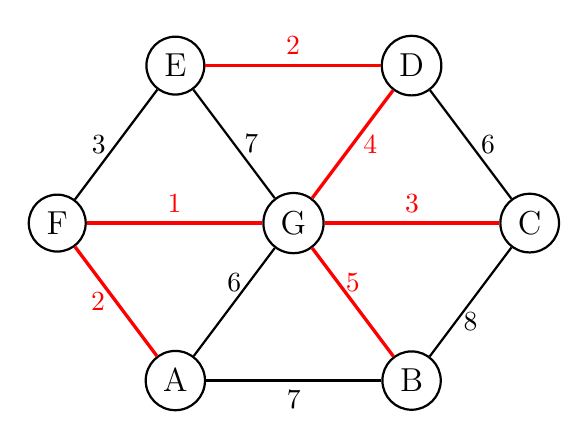
\begin{tikzpicture}
        [node/.style={circle,draw,minimum size=2em, thick, font=\large},
        edge/.style={thick},
        mst/.style={very thick, red}]
        
        % Vertices in a circular arrangement
        \node[node] (A) at (0,0) {A};
        \node[node] (B) at (3,0) {B};
        \node[node] (C) at (4.5,2) {C};
        \node[node] (D) at (3,4) {D};
        \node[node] (E) at (0,4) {E};
        \node[node] (F) at (-1.5,2) {F};
        \node[node] (G) at (1.5,2) {G};
        
        % Non-MST edges (normal black edges)
        \draw[edge] (A) -- (B) node[midway, below] {7};
        \draw[edge] (B) -- (C) node[midway, below] {8};
        \draw[edge] (C) -- (D) node[midway, right] {6};
        \draw[edge] (A) -- (G) node[midway, above] {6};
        \draw[edge] (E) -- (G) node[midway, right] {7};
        \draw[edge] (F) -- (E) node[midway, left] {3};
        
        % MST edges (highlighted in red)
        \draw[mst] (A) -- (F) node[midway, left] {2};
        \draw[mst] (G) -- (D) node[midway, right] {4};
        \draw[mst] (F) -- (G) node[midway, above] {1};
        \draw[mst] (G) -- (C) node[midway, above] {3};
        \draw[mst] (E) -- (D) node[midway, above] {2};
        \draw[mst] (B) -- (G) node[midway, above] {5};
        
    \end{tikzpicture}
    \caption{Um grafo não-dirigido com sete vértices. As arestas em vermelho formam uma árvore geradora mínima (MST) de peso total 17.}
    \label{fig:mst_example}
\end{figure}

Para desenvolver uma árvore geradora mínima, podemos definir uma abordagem gulosa para o problema. Em um algoritmo guloso, precisamos, em cada etapa, fazer a melhor escolha dentre várias possíveis. O programa abaixo ilustra um algoritmo genérico para este problema. 

\begin{programruledcaption}{Função genérica que devolve uma MST de um grafo G.\label{prog:busca}}
    \noindent\textbf{Entrada}: Recebe um grafo conexo não-dirigido $G$.\\
    \textbf{Saída}: Devolve a árvore geradora de custo mínimo de $G$.
    \vspace{-0.5\baselineskip}
    \begin{lstlisting}[
        language={[brazilian]pseudocode},
        style=pseudocode,
        style=wider,
        functions={},
        specialidentifiers={},
        escapeinside={(*@}{@*)},
    ]
    (*@\bfseries\scshape{Função}@*) constrói_MST(G)
        T = $\emptyset$
        (*@\textbf{enquanto}@*) T não formar uma árvore geradora
            encontre uma aresta $uv$ que seja segura à T
            T = A $\cup$ $\{uv\}$
        (*@\textbf{retorne}@*) T
    \end{lstlisting}
    \vspace{-0.5\baselineskip}
\end{programruledcaption}

O método acima administra um conjunto de arestas A, mantendo o seguinte invariante: antes de cada iteração, $T$ é um subconjunto de alguma árvore geradora mínima. Em cada etapa, determinamos uma aresta $uv$ que pode ser adicionada a $T$ sem violar tal invariante, de modo que $T \cup \{uv\}$ também é um subconjunto de uma árvore geradora mínima. Chamamos $uv$ de \textbf{aresta segura} para $T$, visto que ela pode ser adicionada a $T$ e ainda manter o invariante. 

Na linha 1, fica trivial que o conjunto $T$ satisfaz o invariante do laço. Nas linhas 2-4 o invariante é mantido pois estamos adicionando somente arestas seguras. Na linha 5, como $T$ está contido em uma árvore geradora e em uma árvore geradora mínima, então o conjunto $T$ retornado nesta linha deve ser uma árvore geradora mínima. 

Note que o desafio é encontrar a aresta segura da linha 3 do algoritmo. Porém, existem dois algoritmos gulosos que resolvem este problema: o algoritmo de Kruskal e o de Prim. Cada um deles estabelece uma regra específica para determinar uma aresta segura nesta linha 3. No algoritmo de Kruskal, o conjunto $T$ é sempre uma aresta de peso mínimo no grafo que conecta duas componentes distintas. Já no algoritmo de Prim, o conjunto $T$ forma uma árvore única. A aresta segura adicionada a $T$ é sempre uma aresta de peso mínimo que conecta a árvore a um vértice não presente na árvore. Como tais algoritmos são bem descritos no Capítulo 23.2 do livro de Cormen, Leiserson, Rivest e Stein \cite{clrs}, não iremos aprofundá-los em nosso estudo. 

Como se pode perceber, o algoritmo genérico resolve um problema estático em grafos, visto que todas as arestas de um grafo já foram definidas no início do problema. Dessa forma, como não precisamos nos preocupar com alterações no grafo, então ele sempre vai possuir as mesmas árvores geradoras de custo mínimo, ou até somente uma única árvore (quando os pesos das arestas são todos distintos). Em nosso estudo, estamos interessados no problema das florestas geradoras de custo mínimo (FGCM) em grafos dinâmicos, o que implica que a adição ou remoção de uma aresta pode alterar a estrutura das árvores dessas florestas.

Uma floresta é um grafo não-dirigido que não contém nenhum ciclo. É um grafo que pode ser decomposto em várias árvores disjuntas. Dessa forma, quando temos várias árvores disjuntas geradoras de custo mínimo que compõem um grafo, então temos uma floresta geradora de custo mínimo deste grafo. Este problema já existe uma solução proposta por \textit{Holm, de Lichtenberg e Thorup} \cite{jacob_holm}, na Seção 2 de seu artigo. Na Seção 3, os autores propõem a solução do problema da conexidade em um grafo totalmente dinâmico, sem peso nas arestas. Já na Seção 4, é abordado o problema das florestas geradoras de custo mínimo decrementais (\textit{decremental MSF}, de \textit{Minimum Spanning Forest}), onde é descrito um algoritmo eficiente que suporta somente remoções de arestas. Por fim, na Seção 5 é retratado o problema da florestas geradoras de custo mínimo totalmente dinâmicas (\textit{fully dynamic MSF}), onde o algoritmo de FGCM decrementais é transformado em um algoritmo eficiente de FGCM totalmente dinâmicas, que suporta tanto remoções quanto adições de arestas.

No decorrer do nosso estudo, iremos destrinchar a solução dos autores em vários capítulos. No Capítulo 2 descreveremos brevemente o problema da conexidade em florestas dinâmicas. No Capítulo 3: descreveremos as pontos mais relevantes do algoritmo para o problema da conexidade em grafos dinâmicos. No Capítulo 4: descreveremos a nossa implementação do algoritmo para o problema das florestas geradoras de custo mínimo decrementais. No Capítulo 5...

As implementações dos nossos algoritmos da solução de \textit{Holm, de Lichtenberg e Thorup} \cite{jacob_holm} serão feitas utilizando a linguagem \textit{C++}, onde disponibilizamos o código no repositório do \textit{GitHub} \cite{chung2025}.

\pagestyle{mainmatter}
%!TeX root=../tese.tex
%("dica" para o editor de texto: este arquivo é parte de um documento maior)
% para saber mais: https://tex.stackexchange.com/q/78101

%!TeX root=../tese.tex
%("dica" para o editor de texto: este arquivo é parte de um documento maior)
% para saber mais: https://tex.stackexchange.com/q/78101

\chapter{Conexidade em grafos dinâmicos}

\enlargethispage{.8\baselineskip}

Como citado no Capítulo~1, o problema da conexidade em grafos dinâmicos visa construir um algoritmo eficiente que dá suporte a inserções e remoções de arestas e consultas de conexidade entre dois vértices. O algoritmo de Holm, de Lichtenberg e Thorup~\cite{jacob_holm} para este problema de conexidade mantém $\left\lceil \lg n \right\rceil$ florestas dinâmicas do grafo $G$, e utiliza uma biblioteca que será descrita na próxima seção. 

\section{Conexidade em florestas dinâmicas}
\label{sec:dynamic-forest-connectivity}

Rodrigues \cite{arthur}, em sua dissertação do mestrado, estudou, entre outros assuntos, o problema da conexidade em florestas dinâmicas e implementou o algoritmo que foi proposto na Seção~2 do artigo de Holm, de Lichtenberg e Thorup~\cite{jacob_holm}. No Capítulo~2 da sua dissertação, Rodrigues descreve as rotinas principais de sua implementação, que se baseia em \textit{Euler tour trees}, e realiza uma análise minuciosa da complexidade de tempo de cada rotina de sua implementação. Levando isso em conta, optamos por não apresentar uma descrição detalhada desse mesmo algoritmo, e apenas explicar brevemente o que as rotinas principais fazem, ressaltando algumas diferenças da nossa implementação em código em relação à de Rodrigues.  

O problema da conexidade em florestas dinâmicas pode ser considerado uma simplificação do problema de conexidade em grafos dinâmicos, quando o grafo em questão é uma floresta. A biblioteca que usaremos contém os seguintes métodos:

\begin{itemize}
    \item \texttt{\textbf{florestaDinâmica(n)}}: constrói e devolve uma floresta dinâmica $F$ com $n$ vértices e sem arestas;
    \item \texttt{\textbf{conectadosFD(F, u, v)}}: devolve verdadeiro se \textit{u} e \textit{v} estão na mesma componente da floresta $F$ e falso caso contrário;
    \item \texttt{\textbf{adicioneFD(F, u, v)}}: insere uma aresta \textit{uv} na floresta $F$;
    \item \texttt{\textbf{removaFD(u, v)}}: remove a aresta \textit{uv} da floresta $F$.
\end{itemize}


A estrutura de dados principal usada neste algoritmo de Holm, de Lichtenberg e Thorup~para dar suporte eficientes às rotinas acima é uma árvore binária de busca balanceada (ABBB). Dessa forma, a floresta dinâmica é constituída de várias ABBBs. Rodrigues utiliza \textit{treaps} em sua implementação, que são de natureza aleatória. Em nosso caso, utilizamos árvores \textit{splay}, que foram desenvolvidas por \textit{Sleator e Tarjan} \cite{sleator}. Árvores \textit{splay} são árvores binárias de busca (ABBs) que possuem uma rotina extra (além das usuais de busca, inserção e remoção) chamada \textit{splay}, que é acionada ao final de cada operação feita na árvore, de modo que é sempre aplicada ao nó mais profundo visitado. Isso faz com que o custo de uma sequência de $m$ operações (inserção, remoção ou busca) em uma árvore \textit{splay} com $n$ nós seja $\Oh(m\lg n)$, ou seja, o custo amortizado por operação é $\Oh(\lg n)$. Como também já existe bastante literatura sobre árvores \textit{splay}~\cite[Lecture 12]{kozen}, e seu funcionamento interno não afeta a descrição dos algoritmos que descreveremos, não entraremos em detalhes de sua implementação.

Nesse sentido, o resultado é uma implementação em que \texttt{florestaDinâmica(n)} tem custo $\Theta(n)$ e os demais métodos da biblioteca têm custo amortizado $\Oh(\lg n)$.

\section{Estrutura do grafo dinâmico}
\label{sec:dynamic-graph-structure}

Implementar o grafo dinâmico resume-se à construção da seguinte biblioteca de forma eficiente:

\begin{itemize}
    \item \texttt{\textbf{grafoDinâmico(n)}}: contrói e devolve um grafo dinâmico com $n$ vértices e sem arestas;
    \item \texttt{\textbf{conectadosGD(G, u, v)}}: devolve verdadeiro se os vértices $u$ e $v$ estão na mesma componente de $G$ e falso caso contrário;
    \item \texttt{\textbf{adicioneGD(G, u, v)}}: adiciona a aresta $uv$ no grafo $G$;
    \item \texttt{\textbf{removaGD(G, u, v)}}: remove a aresta $uv$ do grafo $G$.
\end{itemize} 

Para entender a base de como cada uma dessas rotinas funcionam, será necessário apresentar a estrutura interna da implementação do grafo para explicar como ele mantém essas estruturas e como elas deixam essas rotinas mais eficientes.

\subsection{Fatiamento do grafo em níveis}
\label{sec:level-slicing}

Na Seção~3.1 do artigo de Holm, de Lichtenberg e Thorup~\cite{jacob_holm}, é apresentada a técnica de fatiar o grafo $G$ em níveis. Cada aresta do grafo possui um nível entre $1$ e $\left\lceil \lg n \right\rceil$, onde $n$ é o número de vértices do grafo $G$. Toda vez que inserimos uma aresta em $G$, ela possuirá o nível $\left\lceil \lg n \right\rceil$, e ele nunca será aumentado. 

Seja $G$ um grafo com $V(G)$ vértices e $E(G)$ arestas. Se $X$ é um conjunto de arestas tal que $\emptyset \neq X \subseteq E(G)$, então dizemos que o subgrafo de $G$ \textbf{induzido} por $X$ é o subgrafo gerador $H$ de $G$ tal que $E(H) = X$. Denotamos, portanto, $H$ como $G[X]$.

Sendo assim, seja $G_i = G[X]$ um grafo onde $X$ é o conjunto das arestas do grafo $G$ de nível menor ou igual a $i$. Para cada nível $i$, manteremos uma floresta maximal $F_i$ de $G_i$. Além disso, vamos manter também, para cada nível $i$, um grafo $R_i$ em forma de listas de adjacências, que guardam apenas arestas de nível $i$ que não estejam em $F_i$. 

Consequentemente, temos que $G_1 \subseteq G_2 \subseteq \cdots \subseteq G_{\left\lceil \lg n \right\rceil}$, para um grafo $G$ de $n$ vértices, e deduzimos que $G = G_{\left\lceil \lg n \right\rceil}$ e que $F_{\left\lceil \lg n \right\rceil}$ é uma floresta maximal de $G$. Dessa maneira, sempre que estivermos realizando alguma operação de alteração ou consulta de conexidade em nosso grafo $G$, estamos também a realizando na floresta $F_{\left\lceil \lg n \right\rceil}$ de $G$.

Com isso, podemos estabelecer algumas invariantes, que são mantidas ao longo das modificações no grafo $G$:

\begin{enumerate}[label=(\Roman*)]
    \item \label{invariant1} $F_i$ é uma floresta maximal de $G_i$ para todo $1 \leq i \leq  \left\lceil \lg n \right\rceil$;
    
    \item \label{invariant2} $F_i \subseteq F_{i+1}$ para todo $1 \leq i \leq \left\lceil \lg n \right\rceil - 1$;
    
    \item \label{invariant3} Cada componente da floresta $F_i$ possui no máximo $2^i$ vértices.
\end{enumerate}

Na Seção~\ref{sec:dynamic-graph-implementation}, descreveremos com mais detalhes como as rotinas da biblioteca funcionam e como cada uma preserva as invariantes acima, de modo a manter a corretude do algoritmo durante toda a sua execução.

Por fim, para simplificar um pouco a notação, iremos escrever $L = \left\lceil \lg n \right\rceil$, isto é, $F_{\left\lceil \lg n \right\rceil}$ passa a ser escrita como $F_{L}$, da mesma forma que $G_L = G_{\left\lceil \lg n \right\rceil}$ e $R_L = R_{\left\lceil \lg n \right\rceil}$.

\subsection{Tipos de arestas do grafo}
\label{sec:dynamic-graph-edge-types}

% O objetivo de fatiar o grafo em  $\left\lceil \lg n \right\rceil$ níveis é para caso uma aresta da floresta de nível $i$ for removida, não será mais necessário procurar exaustivamente por substitutas nos níveis menores que $i$. Assim, passamos a buscar a substituta inicialmente nas arestas reservas em $R_i$. Caso não a encontremos, procuramos nas listas de adjacências $R_{i+1}, R_{i+2}, \ldots, R_{\left\lceil \lg n \right\rceil}$. Se não existir uma aresta substituta em $R_j$, $i \leq j \leq  \left\lceil \lg n \right\rceil$, então rebaixaremos as arestas que exploramos em $R_j$ de nível $j$ para um nível inferior $j-1$, caso $j > 0$. 

Quando realizamos uma chamada à função \texttt{adicioneGD(G, u, v)}, é feita uma chamada à rotina \texttt{conectadosGD(G, u, v)} para verificar a conexidade de $u$ com $v$ em $G$. Se estes vértices não estiverem ligados em $G$, então a aresta $uv$ é inserida na floresta maximal $F_L$ que estamos mantendo, assim ligando a árvore que contém $u$ com a que contém $v$ em $F_L$. Chamamos esse tipo de aresta de \textbf{arestas da floresta}.

Caso $u$ e $v$ já estejam conectados em $G$, então essa aresta $uv$ é chamada de \textbf{aresta reserva} e ela será armazenada no grafo $R_L$ representado por listas de adjacências, que contém a seguinte biblioteca:

\begin{itemize}
    \item \texttt{\textbf{listaDeAdjacências(n)}}: constrói e devolve um grafo com $n$ vértices e sem arestas representado por listas de adjacências;
    \item \texttt{\textbf{adicioneLA(R, u, v)}}: adiciona $u$ na lista de adjacências de $v$ em $R$ e vice-versa;
    \item \texttt{\textbf{removaLA(R, u, v)}}: remove $u$ da lista de adjacências de $v$ em $R$ e vice-versa.
\end{itemize} 

A nossa implementação \cite{chung2025} de listas de adjacências possui um custo $\Oh(n)$ ao acionar o construtor \texttt{listaDeAdjacências}, e para 
as rotinas \texttt{adicioneLA} e \texttt{removaLA} é garantido tempo esperado $\Oh(1)$, visto que estamos utilizando um mapa hash da linguagem \textit{C++} para realizar adição de um vizinho $v$ na lista de $u$ e, remoção de $v$ da lista de adjacências de $u$.

\section{Rotinas da biblioteca do grafo dinâmico}

\subsection{Criação do grafo}
\label{sec:dynamic-graph-creation}

Para criar o grafo dinâmico $G$ com $n$ vértices e sem arestas, chamamos a rotina \texttt{grafoDinâmico(n)}, que por sua vez irá chamar \texttt{florestaDinâmica(n)}, inicializando $\left\lceil \lg n \right\rceil$ florestas dinâmicas de $n$ vértices isolados, e \texttt{listaDeAdjacências(n)}, inicializando $\left\lceil \lg n \right\rceil$ listas de adjacências de $n$ vértices isolados. Como as duas últimas rotinas consomem tempo $\Oh(n)$, então \texttt{grafoDinâmico} consome tempo $\Oh(n \lg n)$.

\subsection{Consultas de conexidade no grafo dinâmico}
\label{sec:dynamic-graph-connectivity-queries}

Para testar a conexidade entre dois vértices $u$ e $v$ no grafo $G$, basta chamarmos \texttt{conectadosGD(G, u, v)}, que por sua vez irá devolver a resposta de \texttt{conectadosFD($F_L$, u, v)}, pois $F_L$ é a floresta maximal de $G$. A rotina \texttt{conectadosFD($F_L$, u, v)} em nossa implementação consome tempo amortizado $\Oh(\lg n)$, e, portanto, \texttt{conectadosGD($F_L$, u, v)} também terá o mesmo consumo de tempo amortizado.

\subsection{Inserções de arestas no grafo dinâmico}

Como explicado na Seção~\ref{sec:dynamic-graph-edge-types}, inserimos uma aresta $uv$ no grafo $G$ chamando a rotina \texttt{adicioneGD(G, u, v)}, e, em seguida, testamos a conexidade de $u$ e $v$ chamando a rotina \texttt{conectadosGD(G, u, v)}, que dependendo do resultado $uv$ pode ser inserida como aresta reserva ou aresta da floresta. Assumindo que a aresta $uv$ não exista na floresta maximal $F_L$ de $G$ no momento de sua inserção, temos dois cenários:

\begin{itemize}
    \item 
    Se os vértices $u$ e $v$ já estão conectados, então iremos chamar a função \texttt{adicioneLA($R_L$, u, v)}, que irá armazenar $uv$ como aresta reserva de nível $L$ de $G$ em $R_L$. A Figura~\ref{fig:graph_reserve_edge_uv_addition} ilustra esse cenário.

\end{itemize}

\begin{figure}[H]
    \centering
    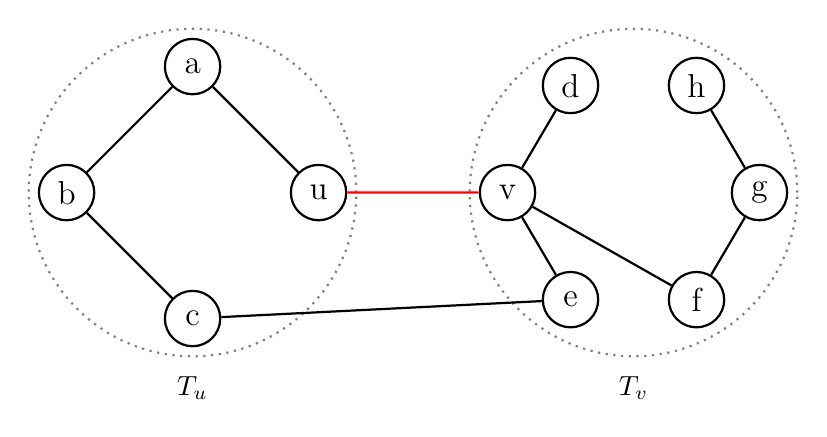
\begin{tikzpicture}
        [scale=0.8, node/.style={circle,draw,minimum size=2em, thick, font=\large},
        edge/.style={thick, black},
        reserve/.style={red, thick},
        removed/.style={black, thick, dashed}]

        \node[node] (u) at (-1,2) {u};
        \node[node] (a) at (-3,4) {a};
        \node[node] (b) at (-5,2) {b};
        \node[node] (c) at (-3,0) {c};
        \node[node] (v) at (2,2) {v};
        \node[node] (d) at (3,3.7) {d};
        \node[node] (e) at (3,0.3) {e};
        \node[node] (f) at (5,0.3) {f};
        \node[node] (g) at (6, 2) {g};
        \node[node] (h) at (5, 3.7) {h};
        
        
         % Dotted circles for T_u and T_v
        \draw[dotted, thick, gray] (-3,2) circle (2.6cm);
        \draw[dotted, thick, gray] (4,2) circle (2.6cm);  
        
        % Labels for the circles
        \node at (-3,-1.1) {$T_u$};
        \node at (4,-1.1) {$T_v$};

        % tree edges (normal black edges)
        \draw[edge] (a) -- (u) node[midway, below] {};
        \draw[edge] (a) -- (b) node[midway, below] {};
        \draw[edge] (b) -- (c) node[midway, below] {};
        \draw[edge] (v) -- (d) node[midway, below] {};
        \draw[edge] (v) -- (f) node[midway, below] {};
        \draw[edge] (v) -- (e) node[midway, below] {};
        \draw[edge] (c) -- (e) node[midway, below] {};
        \draw[edge] (f) -- (g) node[midway, below] {};
        \draw[edge] (g) -- (h) node[midway, below] {};

        % reserve edges (normal red edges)
        \draw[reserve] (u) -- (v) node[midway, below] {};


    \end{tikzpicture}
    \caption{As arestas pretas são da floresta maximal $F_L$ do grafo. Como queremos inserir a aresta $uv$ e os vértices $u$ e $v$ já estão conectados pelo caminho $u \rightarrow a \rightarrow b \rightarrow c \rightarrow e \rightarrow v$, então armazenamos $uv$ como aresta reserva (em vermelho).}
    \label{fig:graph_reserve_edge_uv_addition}
\end{figure}

\begin{itemize}
    \item  Se $u$ e $v$ não estão conectados por nenhum caminho em $G$, então inserimos $uv$ como aresta de floresta de nível $L$ em $F_L$ chamando a função \texttt{adicioneFD($F_L$, u, v)}. A Figura~\ref{fig:graph_tree_edge_uv_addition} ilustra esse cenário.
\end{itemize}

\begin{figure}[H]
    \centering
    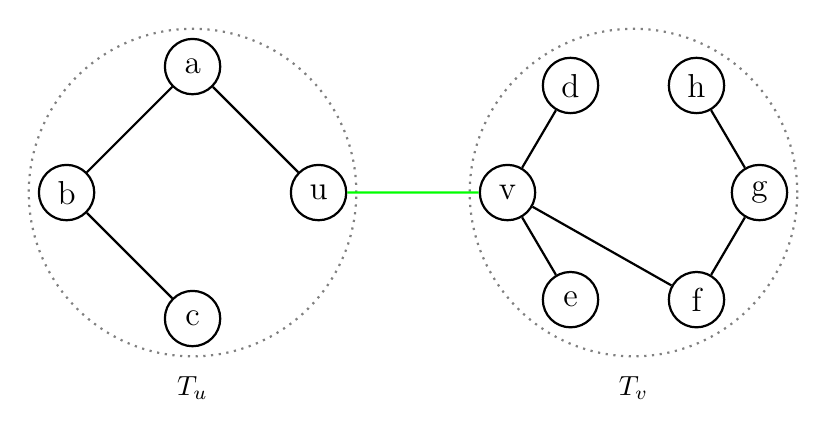
\begin{tikzpicture}
        [scale=0.8, node/.style={circle,draw,minimum size=2em, thick, font=\large},
        edge/.style={thick, black},
        added/.style={thick, green},
        reserve/.style={red, thick},
        removed/.style={black, thick, dashed}]

        \node[node] (u) at (-1,2) {u};
        \node[node] (a) at (-3,4) {a};
        \node[node] (b) at (-5,2) {b};
        \node[node] (c) at (-3,0) {c};
        \node[node] (v) at (2,2) {v};
        \node[node] (d) at (3,3.7) {d};
        \node[node] (e) at (3,0.3) {e};
        \node[node] (f) at (5,0.3) {f};
        \node[node] (g) at (6, 2) {g};
        \node[node] (h) at (5, 3.7) {h};
        
        
         % Dotted circles for T_u and T_v
        \draw[dotted, thick, gray] (-3,2) circle (2.6cm);
        \draw[dotted, thick, gray] (4,2) circle (2.6cm);  
        
        % Labels for the circles
        \node at (-3,-1.1) {$T_u$};
        \node at (4,-1.1) {$T_v$};

        % tree edges (normal black edges)
        \draw[edge] (a) -- (u) node[midway, below] {};
        \draw[edge] (a) -- (b) node[midway, below] {};
        \draw[edge] (b) -- (c) node[midway, below] {};
        \draw[edge] (v) -- (d) node[midway, below] {};
        \draw[edge] (v) -- (f) node[midway, below] {};
        \draw[edge] (v) -- (e) node[midway, below] {};
        \draw[edge] (f) -- (g) node[midway, below] {};
        \draw[edge] (g) -- (h) node[midway, below] {};
        \draw[added] (u) -- (v) node[midway, below] {};

        % reserve edges (normal red edges)


    \end{tikzpicture}
    \caption{As arestas pretas são da floresta maximal $F_L$ do grafo. Como os vértices $u$ e $v$ não estão conectados, então inserimos $uv$ como aresta da floresta (em verde), nesse caso conectando as componentes $T_u$ e $T_v$.}
    \label{fig:graph_tree_edge_uv_addition}
\end{figure}

Em nossa implementação, \texttt{conectadosGD} consome tempo amortizado $\Oh(\lg n)$. A rotina \texttt{adicioneLA}, quando acionada, consome tempo esperado constante $\Oh(1)$ em nossa implementação por conta do mapa \textit{hash}. Já inserir uma aresta da floresta chamando \texttt{adicioneFD} consome tempo $\Oh(\lg n)$ (amortizado, em nossa implementação). Portanto, o custo de tempo ao acionar a rotina \texttt{adicioneGD} será amortizado $\Oh(\lg n)$.























































\subsection{Remoção de arestas no grafo dinâmico}
\label{sec:dynamic-graph-edge-removal}

A remoção de arestas se divide em dois casos: remoção de uma aresta reserva ou remoção de uma aresta da floresta.

Quando queremos remover uma aresta $uv$ e ela é reserva, podemos simplesmente acionar a rotina \texttt{removaLA($R_i$, u, v)} onde $i$ é o nível da aresta a ser removida e $R_i$ a lista de adjacências na qual ela está armazenada. Por conta disso, a floresta maximal $F_L$ do grafo não será afetada. A Figura~\ref{fig:graph_reserve_edge_removal} mostra esse cenário apresentado.

\begin{figure}[H]
    \centering
    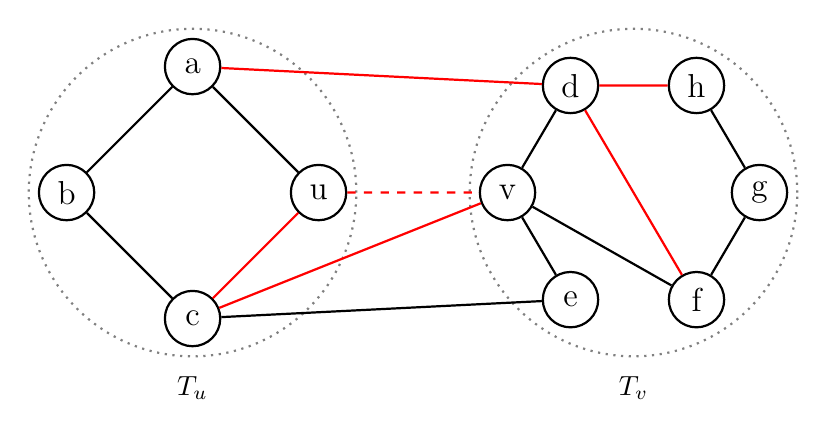
\begin{tikzpicture}
        [scale=0.8, node/.style={circle,draw,minimum size=2em, thick, font=\large},
        edge/.style={thick, black},
        reserve/.style={red, thick},
        removed/.style={black, thick, dashed},
        removed_reserve/.style={red, thick, dashed}]

        \node[node] (u) at (-1,2) {u};
        \node[node] (a) at (-3,4) {a};
        \node[node] (b) at (-5,2) {b};
        \node[node] (c) at (-3,0) {c};
        \node[node] (v) at (2,2) {v};
        \node[node] (d) at (3,3.7) {d};
        \node[node] (e) at (3,0.3) {e};
        \node[node] (f) at (5,0.3) {f};
        \node[node] (g) at (6, 2) {g};
        \node[node] (h) at (5, 3.7) {h};
        
        
         % Dotted circles for T_u and T_v
        \draw[dotted, thick, gray] (-3,2) circle (2.6cm);
        \draw[dotted, thick, gray] (4,2) circle (2.6cm);  
        
        % Labels for the circles
        \node at (-3,-1.1) {$T_u$};
        \node at (4,-1.1) {$T_v$};

        % tree edges (normal black edges)
        \draw[edge] (a) -- (u) node[midway, below] {};
        \draw[edge] (a) -- (b) node[midway, below] {};
        \draw[edge] (b) -- (c) node[midway, below] {};
        \draw[edge] (v) -- (d) node[midway, below] {};
        \draw[edge] (v) -- (f) node[midway, below] {};
        \draw[edge] (v) -- (e) node[midway, below] {};
        \draw[edge] (c) -- (e) node[midway, below] {};
        \draw[edge] (f) -- (g) node[midway, below] {};
        \draw[edge] (g) -- (h) node[midway, below] {};

        % reserve edges (normal red edges)
        \draw[reserve] (a) -- (d) node[midway, below] {};
        \draw[reserve] (c) -- (v) node[midway, below] {};
        \draw[removed_reserve] (u) -- (v) node[midway, below] {};
        \draw[reserve] (c) -- (u) node[midway, below] {};
        \draw[reserve] (d) -- (f) node[midway, below] {};
        \draw[reserve] (d) -- (h) node[midway, below] {};

    \end{tikzpicture}
    \caption{As arestas pretas são da floresta maximal $F_L$ do grafo, enquanto as vermelhas são arestas reservas. A aresta vermelha $uv$ tracejada é reserva e está prestes a ser removida.}
    \label{fig:graph_reserve_edge_removal}
\end{figure}

O caso da remoção de uma aresta $uv$ da floresta é mais complexo. Se o grafo no qual queremos fazer a remoção possuir somente uma componente, remover $uv$ iria acabar quebrando ela em duas componentes, as quais chamaremos de árvores $T_u$ e $T_v$, de modo que a primeira contém o vértice $u$ e a segunda contém o vértice $v$. Neste caso, precisamos verificar se existe alguma aresta reserva que ligue $T_u$ à $T_v$, para que possamos garantir que a floresta $F_L $ continue maximal em $G$. Assim, precisamos procurar uma aresta reserva para substituir a aresta que foi removida de $G$, que vamos chamar de \textbf{aresta substituta}.

\begin{figure}[H]
    \centering
    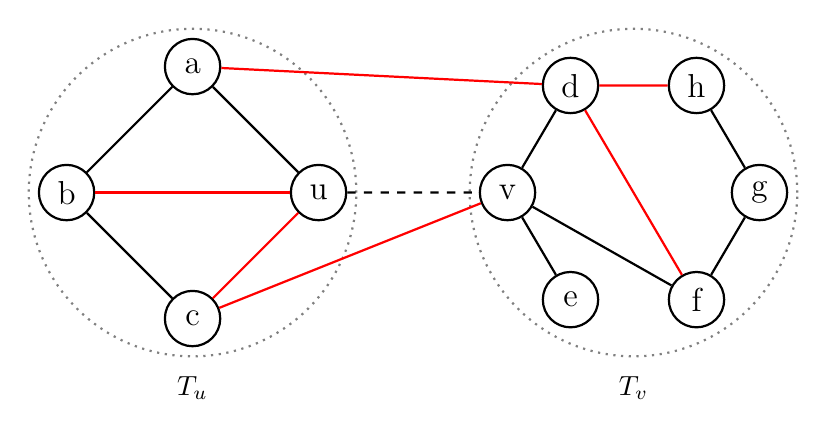
\begin{tikzpicture}
        [scale=0.8, node/.style={circle,draw,minimum size=2em, thick, font=\large},
        edge/.style={thick, black},
        reserve/.style={red, thick},
        removed/.style={black, thick, dashed}]

        \node[node] (u) at (-1,2) {u};
        \node[node] (a) at (-3,4) {a};
        \node[node] (b) at (-5,2) {b};
        \node[node] (c) at (-3,0) {c};
        \node[node] (v) at (2,2) {v};
        \node[node] (d) at (3,3.7) {d};
        \node[node] (e) at (3,0.3) {e};
        \node[node] (f) at (5,0.3) {f};
        \node[node] (g) at (6, 2) {g};
        \node[node] (h) at (5, 3.7) {h};
        
        
         % Dotted circles for T_u and T_v
        \draw[dotted, thick, gray] (-3,2) circle (2.6cm);
        \draw[dotted, thick, gray] (4,2) circle (2.6cm);  
        
        % Labels for the circles
        \node at (-3,-1.1) {$T_u$};
        \node at (4,-1.1) {$T_v$};

        % tree edges (normal black edges)
        \draw[edge] (a) -- (u) node[midway, below] {};
        \draw[edge] (a) -- (b) node[midway, below] {};
        \draw[edge] (b) -- (c) node[midway, below] {};
        \draw[edge] (v) -- (d) node[midway, below] {};
        \draw[edge] (v) -- (f) node[midway, below] {};
        \draw[edge] (v) -- (e) node[midway, below] {};
        \draw[removed] (u) -- (v) node[midway, above] {};
        \draw[edge] (f) -- (g) node[midway, below] {};
        \draw[edge] (g) -- (h) node[midway, below] {};
        \draw[reserve] (a) -- (d) node[midway, below] {};
        \draw[reserve] (c) -- (v) node[midway, below] {};

        % reserve edges (normal red edges)
        \draw[reserve] (b) -- (u) node[midway, below] {};
        \draw[reserve] (c) -- (u) node[midway, below] {};
        \draw[reserve] (d) -- (f) node[midway, below] {};
        \draw[reserve] (d) -- (h) node[midway, below] {};

    \end{tikzpicture}
    \caption{As arestas pretas são da floresta maximal $F_L$ do grafo, enquanto as vermelhas são reservas. A aresta $uv$ tracejada está prestes a ser removida e substituída pela $ad$ ou $cv$, pois qualquer uma destas liga $T_u$ à $T_v$.}
    \label{fig:graph_with_Tu_and_Tv_with_reserve_edge}
\end{figure}

Podemos supor, sem perda de generalidade, que o número de vértices de $T_u$ é no máximo o de $T_v$. Assim, para procurar uma aresta reserva que substitua a removida, vamos percorrer cada vértice $x$ de $T_u$ e verificar se existe algum vértice $y$ na lista de adjacências de $x$, de modo que $y$ esteja em $T_v$. Se $y \in V(T_v)$, então a aresta $xy$ é uma aresta substituta, bastando apenas acionar \texttt{adicioneFD(F, x, y)} para reconectar $T_u$ e $T_v$, que virariam uma única componente da floresta $F_L$.

Note que procurar todas as arestas que tenham a ponta em algum vértice de $T_u$ pode ser custoso, visto que $V(T_u)$ é da ordem de $\Oh(n)$, onde $n$ é o número de vértices do grafo $G$. É por este motivo que introduzimos o fatiamento em níveis na Seção~\ref{sec:level-slicing}. A intuição por trás deste fatiamento é que, quando uma aresta da floresta de nível $i$ é removida, não é necessário buscar por substitutas nos níveis menores que $i$. Isso quer dizer que começamos a busca no nível em questão, ou seja, $R_i$, e caso nesta lista de adjacências não haja nenhuma substituta, passamos a procurar em $R_{i+1}, R_{i + 2}, \ldots, R_L$. Quando não encontramos uma substituta em um certo $R_j$, aproveitamos para rebaixar o nível de todas as arestas percorridas em $R_j$ para $j - 1$, $j > 1$, de modo que não precisaremos mais percorrer essas arestas quando removermos uma outra aresta de nível $j$, visto que elas já estariam em $R_{j-1}$.

+++++++++ PORQUE NAO PROCURAR SUBSTITUTA EM NIVEL < i ++++++++++

O motivo de não precisarmos procurar uma substituta em níveis menores que $i$ quando removemos uma aresta $uv$ de nível $i$ é devido à invariantes~\ref{invariant1} e \ref{invariant2}. Vamos provar esse fato por contradição, supondo inicialmente que exista uma aresta $xy$ de nível $j < i$ que substitua $uv$. Como $xy$ é uma aresta de nível $j$, temos que $xy \in E(G_{j})$, e, portanto, os vértices $x$ e $y$ estão na mesma componente de $G_j$. Pela invariante~\ref{invariant1}, $F_j$ é uma floresta maximal de $G_j$, o que implica que $x$ e $y$ estão na mesma componente conexa de $F_j$. Pela invariante~\ref{invariant2}, temos $F_{j} \subseteq F_{i}$ ... 

+++++++++++++++++++++++++++++++++++++++++++++++++++++++++++++

A seguir, iremos demonstrar a remoção de uma aresta $uv$ da floresta em uma série de imagens. Na Figura~\ref{fig:example-replacement1}, temos um grafo $G$ de $n = 10$ vértices. Para facilitar, iremos assumir que, até o momento, só houve inserções de arestas. Temos também que $n = 10$, $\left\lceil \lg 10 \right\rceil = 4$, logo o nível máximo $L$ da floresta é $4$, e consequentemente, $G = G_4$. Como todas as inserções só acontecem no nível $L$, no momento só temos arestas da floresta de nível $4$ em $F_4$ de $G$, enquanto $F_3$ contém apenas vértices isolados. Neste cenário, note que 
a remoção da aresta $uv$ da floresta (representada por uma linha tracejada na figura) acaba quebrando a única componente da floresta em duas, $T_u$ e $T_v$. 

\begin{figure}[H]
    \centering

    \noindent
    \begin{minipage}[c]{2cm}
        \raggedright
        Nível $4$
    \end{minipage}%
    \begin{minipage}[c]{0.8\textwidth}
        \centering
        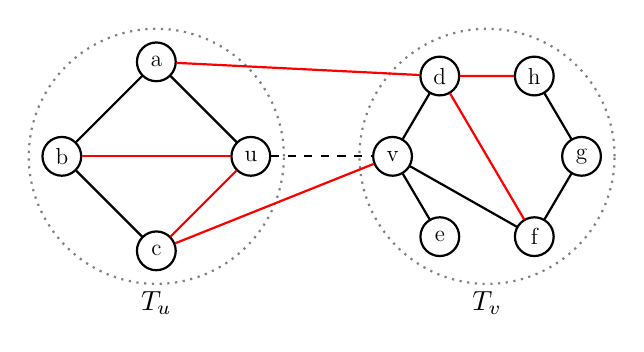
\begin{tikzpicture}
        [scale=0.6, node/.style={scale=0.7, circle,draw,minimum size=2em, thick, font=\large},
        edge/.style={thick, black},
        reserve/.style={red, thick},
        removed/.style={black, thick, dashed}]

        \node[node] (u) at (-1,2) {u};
        \node[node] (a) at (-3,4) {a};
        \node[node] (b) at (-5,2) {b};
        \node[node] (c) at (-3,0) {c};
        \node[node] (v) at (2,2) {v};
        \node[node] (d) at (3,3.7) {d};
        \node[node] (e) at (3,0.3) {e};
        \node[node] (f) at (5,0.3) {f};
        \node[node] (g) at (6, 2) {g};
        \node[node] (h) at (5, 3.7) {h};
        
         % Dotted circles for T_u and T_v
        \draw[dotted, thick, gray] (-3,2) circle (2.7cm);
        \draw[dotted, thick, gray] (4,2) circle (2.7cm);  
        
        % Labels for the circles
        \node at (-3,-1.1) {$T_u$};
        \node at (4,-1.1) {$T_v$};

        % tree edges (normal black edges)
        \draw[edge] (a) -- (u) node[midway, below] {};
        \draw[edge] (a) -- (b) node[midway, below] {};
        \draw[edge] (b) -- (c) node[midway, below] {};
        \draw[edge] (v) -- (d) node[midway, below] {};
        \draw[edge] (v) -- (f) node[midway, below] {};
        \draw[edge] (v) -- (e) node[midway, below] {};
        \draw[edge] (f) -- (g) node[midway, below] {};
        \draw[edge] (g) -- (h) node[midway, below] {};
        % reserve edges (normal red edges)
        
        \draw[removed] (u) -- (v) node[midway, below] {};
        \draw[reserve] (a) -- (d) node[midway, below] {};
        \draw[reserve] (c) -- (v) node[midway, below] {};
        \draw[reserve] (b) -- (u) node[midway, below] {};
        \draw[reserve] (c) -- (u) node[midway, below] {};
        \draw[reserve] (d) -- (f) node[midway, below] {};
        \draw[reserve] (d) -- (h) node[midway, below] {};

        \end{tikzpicture}
    \end{minipage}
    \vspace{1cm}
        \noindent
    \begin{minipage}[c]{2cm}
        \raggedright
        Nível $3$
    \end{minipage}%
    \begin{minipage}[c]{0.8\textwidth}
        \centering
        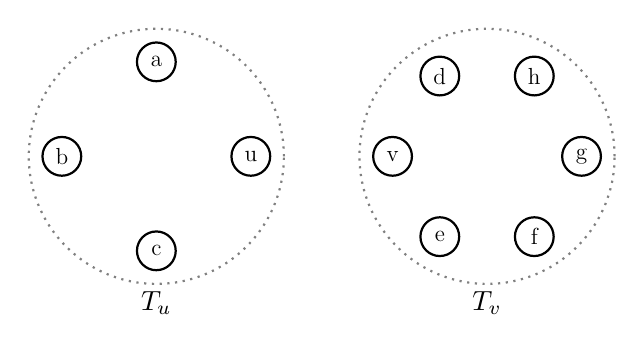
\begin{tikzpicture}
            [scale=0.6, node/.style={scale=0.7, circle,draw,minimum size=2em, thick, font=\large},
            edge/.style={thick, black},
            reserve/.style={red, thick},
            removed/.style={black, thick, dashed}]

            \node[node] (u) at (-1,2) {u};
            \node[node] (a) at (-3,4) {a};
            \node[node] (b) at (-5,2) {b};
            \node[node] (c) at (-3,0) {c};
            \node[node] (v) at (2,2) {v};
            \node[node] (d) at (3,3.7) {d};
            \node[node] (e) at (3,0.3) {e};
            \node[node] (f) at (5,0.3) {f};
            \node[node] (g) at (6, 2) {g};
            \node[node] (h) at (5, 3.7) {h};
            
            
            % Dotted circles for T_u and T_v
            \draw[dotted, thick, gray] (-3,2) circle (2.7cm);
            \draw[dotted, thick, gray] (4,2) circle (2.7cm);  
            
            % Labels for the circles
            \node at (-3,-1.1) {$T_u$};
            \node at (4,-1.1) {$T_v$};
            
            %\draw[edge] (a) -- (u) node[midway, below] {};
            %\draw[edge] (a) -- (b) node[midway, below] {};
            %\draw[edge] (b) -- (c) node[midway, below] {};

        \end{tikzpicture}
    \end{minipage}
    \caption{Um grafo $G$ de 10 vértices, onde as arestas pretas são da floresta, enquanto as vermelhas são reservas. A aresta $uv$ está prestes a ser removida. A floresta $F_{i = 4}$ de $G$ de cima contém todas as arestas recém-inseridas, enquanto a de baixo é a $F_{i = 3}$, com os vértices isolados.}
    \vspace{-1cm}
    \label{fig:example-replacement1}
\end{figure}

Note que precisamos remover todas as arestas $uv$ que estão presentes no nível $i = 4$ e os que estão acima dele também, por conta da invariante~\ref{invariant2}. Como $F_4$ é a floresta maximal de nível máximo de $G$, então removemos somente a $uv$ de $F_4$. 

O próximo passo é rebaixar o nível de todas as arestas de nível $4$ em $T_u$. Rebaixar o nível das arestas significa inserir as arestas de nível $4$ de $T_u$ em $F_3$, onde elas passam a ser de nível $3$. Esse rebaixamento se torna necessário para preservar a invariante~\ref{invariant3}. Denotando $|T|$ como o número de vértices de uma árvore $T$, podemos, sem perda de generalidade, assumir que $|T_u| \leq |T_v|$. Pela invariante~\ref{invariant3}, temos que $|T| \leq 2^i$, e como $|T_u| + |T_v| = |T|$, então $|T_u| \leq 2^{i-1}$. Por isso, rebaixamos todas as arestas de nível $i$ de $T_u$ para o nível $i-1$, mantendo-se, assim, a invariante. 

Perceba que, devido à invariante~\ref{invariant2}, podemos ter arestas de diferentes níveis em uma mesma árvore. Assim, percorrer todas as arestas da floresta de $T_u$ e selecionar somente as de nível $i$ para rebaixar pode se tornar muito demorado quando o grafo possui uma enorme quantidade de arestas. A forma como o algoritmo procura as arestas de nível $i$ será descrita de maneira mais detalhada a nível de código na Seção~\ref{sec:code-edge-removal}. No momento, só precisamos entender como este rebaixamento funciona.

\begin{figure}[H]
    \centering

    \noindent
    \begin{minipage}[c]{2cm}
        \raggedright
        Nível $4$
    \end{minipage}%
    \begin{minipage}[c]{0.8\textwidth}
        \centering
        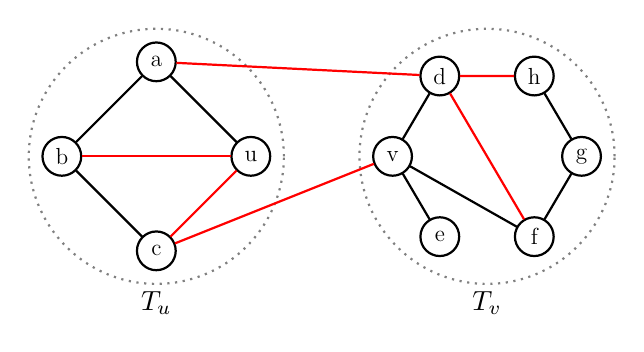
\begin{tikzpicture}
        [scale=0.6, node/.style={scale=0.7, circle,draw,minimum size=2em, thick, font=\large},
        edge/.style={thick, black},
        reserve/.style={red, thick},
        removed/.style={black, thick, dashed}]

        \node[node] (u) at (-1,2) {u};
        \node[node] (a) at (-3,4) {a};
        \node[node] (b) at (-5,2) {b};
        \node[node] (c) at (-3,0) {c};
        \node[node] (v) at (2,2) {v};
        \node[node] (d) at (3,3.7) {d};
        \node[node] (e) at (3,0.3) {e};
        \node[node] (f) at (5,0.3) {f};
        \node[node] (g) at (6, 2) {g};
        \node[node] (h) at (5, 3.7) {h};
        
         % Dotted circles for T_u and T_v
        \draw[dotted, thick, gray] (-3,2) circle (2.7cm);
        \draw[dotted, thick, gray] (4,2) circle (2.7cm);  
        
        % Labels for the circles
        \node at (-3,-1.1) {$T_u$};
        \node at (4,-1.1) {$T_v$};

        % tree edges (normal black edges)
        \draw[edge] (a) -- (u) node[midway, below] {};
        \draw[edge] (a) -- (b) node[midway, below] {};
        \draw[edge] (b) -- (c) node[midway, below] {};
        \draw[edge] (v) -- (d) node[midway, below] {};
        \draw[edge] (v) -- (f) node[midway, below] {};
        \draw[edge] (v) -- (e) node[midway, below] {};
        \draw[edge] (f) -- (g) node[midway, below] {};
        \draw[edge] (g) -- (h) node[midway, below] {};
        % reserve edges (normal red edges)
        
        \draw[reserve] (a) -- (d) node[midway, below] {};
        \draw[reserve] (c) -- (v) node[midway, below] {};
        \draw[reserve] (b) -- (u) node[midway, below] {};
        \draw[reserve] (c) -- (u) node[midway, below] {};
        \draw[reserve] (d) -- (f) node[midway, below] {};
        \draw[reserve] (d) -- (h) node[midway, below] {};

        \end{tikzpicture}
    \end{minipage}
    \vspace{1cm}
        \noindent
    \begin{minipage}[c]{2cm}
        \raggedright
        Nível $3$
    \end{minipage}%
    \begin{minipage}[c]{0.8\textwidth}
        \centering
        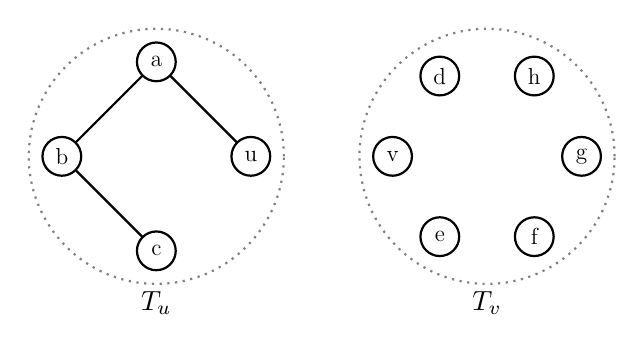
\begin{tikzpicture}
            [scale=0.6, node/.style={scale=0.7, circle,draw,minimum size=2em, thick, font=\large},
            edge/.style={thick, black},
            reserve/.style={red, thick},
            removed/.style={black, thick, dashed}]

            \node[node] (u) at (-1,2) {u};
            \node[node] (a) at (-3,4) {a};
            \node[node] (b) at (-5,2) {b};
            \node[node] (c) at (-3,0) {c};
            \node[node] (v) at (2,2) {v};
            \node[node] (d) at (3,3.7) {d};
            \node[node] (e) at (3,0.3) {e};
            \node[node] (f) at (5,0.3) {f};
            \node[node] (g) at (6, 2) {g};
            \node[node] (h) at (5, 3.7) {h};
            
            
            % Dotted circles for T_u and T_v
            \draw[dotted, thick, gray] (-3,2) circle (2.7cm);
            \draw[dotted, thick, gray] (4,2) circle (2.7cm);  
            
            % Labels for the circles
            \node at (-3,-1.1) {$T_u$};
            \node at (4,-1.1) {$T_v$};
            
            \draw[edge] (a) -- (u) node[midway, below] {};
            \draw[edge] (a) -- (b) node[midway, below] {};
            \draw[edge] (b) -- (c) node[midway, below] {};

        \end{tikzpicture}
    \end{minipage}
    \caption{Representação da remoção da aresta $uv$ em $G$. As arestas da floresta de nível $4$ de $T_u$ foram rebaixadas para o nível $3$, que podem ser vistas na floresta $F_{3}$.}
    \vspace{-1cm}
    \label{fig:example-replacement2}    
\end{figure}

\raggedbottom

Como $T_u$ e $T_v$ em $F_4$ ficaram separadas após a remoção de $uv$, precisamos achar, se existir, uma aresta reserva que possa reconectá-las. Note que percorrer todas as arestas reservas para achar uma substituta que ligue $T_u$ à $T_v$ pode ser ineficiente quando temos muitas arestas reservas. Por isso, explicaremos como implementar essa busca pela substituta de forma eficiente na Seção~\ref{sec:code-edge-removal}. 


\begin{figure}[H]
    \centering

    \noindent
    \begin{minipage}[c]{2cm}
        \raggedright
        Nível $4$
    \end{minipage}%
    \begin{minipage}[c]{0.8\textwidth}
        \centering
        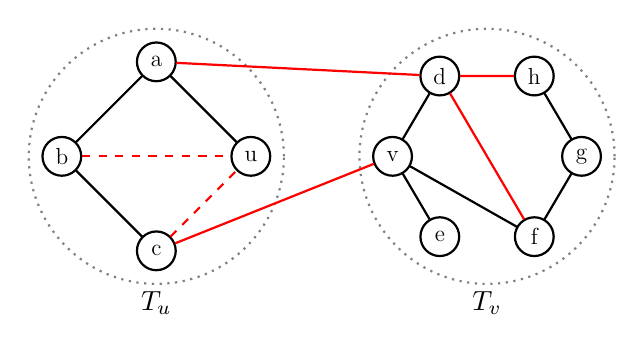
\begin{tikzpicture}
        [scale=0.6, node/.style={scale=0.7, circle,draw,minimum size=2em, thick, font=\large},
        edge/.style={thick, black},
        reserve/.style={red, thick},
        removed/.style={black, thick, dashed}, 
        reserveremoved/.style={red, thick, dashed}]

        \node[node] (u) at (-1,2) {u};
        \node[node] (a) at (-3,4) {a};
        \node[node] (b) at (-5,2) {b};
        \node[node] (c) at (-3,0) {c};
        \node[node] (v) at (2,2) {v};
        \node[node] (d) at (3,3.7) {d};
        \node[node] (e) at (3,0.3) {e};
        \node[node] (f) at (5,0.3) {f};
        \node[node] (g) at (6, 2) {g};
        \node[node] (h) at (5, 3.7) {h};
        
         % Dotted circles for T_u and T_v
        \draw[dotted, thick, gray] (-3,2) circle (2.7cm);
        \draw[dotted, thick, gray] (4,2) circle (2.7cm);  
        
        % Labels for the circles
        \node at (-3,-1.1) {$T_u$};
        \node at (4,-1.1) {$T_v$};

        % tree edges (normal black edges)
        \draw[edge] (a) -- (u) node[midway, below] {};
        \draw[edge] (a) -- (b) node[midway, below] {};
        \draw[edge] (b) -- (c) node[midway, below] {};
        \draw[edge] (v) -- (d) node[midway, below] {};
        \draw[edge] (v) -- (f) node[midway, below] {};
        \draw[edge] (v) -- (e) node[midway, below] {};
        \draw[edge] (f) -- (g) node[midway, below] {};
        \draw[edge] (g) -- (h) node[midway, below] {};
        % reserve edges (normal red edges)
        
        \draw[reserve] (a) -- (d) node[midway, below] {};
        \draw[reserve] (c) -- (v) node[midway, below] {};
        \draw[reserveremoved] (b) -- (u) node[midway, below] {};
        \draw[reserveremoved] (c) -- (u) node[midway, below] {};
        \draw[reserve] (d) -- (f) node[midway, below] {};
        \draw[reserve] (d) -- (h) node[midway, below] {};

        \end{tikzpicture}
    \end{minipage}
    \vspace{1cm}
        \noindent
    \begin{minipage}[c]{2cm}
        \raggedright
        Nível $3$
    \end{minipage}%
    \begin{minipage}[c]{0.8\textwidth}
        \centering
        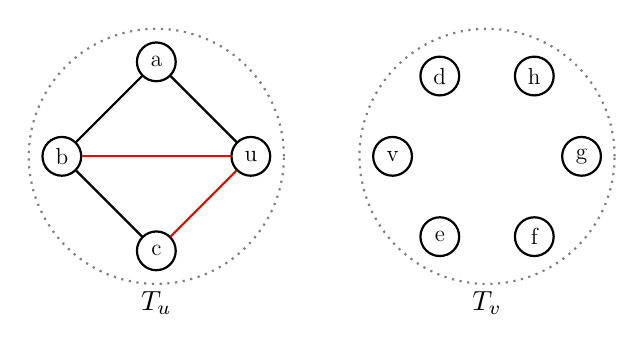
\begin{tikzpicture}
            [scale=0.6, node/.style={scale=0.7, circle,draw,minimum size=2em, thick, font=\large},
            edge/.style={thick, black},
            reserve/.style={red, thick},
            removed/.style={black, thick, dashed}]

            \node[node] (u) at (-1,2) {u};
            \node[node] (a) at (-3,4) {a};
            \node[node] (b) at (-5,2) {b};
            \node[node] (c) at (-3,0) {c};
            \node[node] (v) at (2,2) {v};
            \node[node] (d) at (3,3.7) {d};
            \node[node] (e) at (3,0.3) {e};
            \node[node] (f) at (5,0.3) {f};
            \node[node] (g) at (6, 2) {g};
            \node[node] (h) at (5, 3.7) {h};
            
            
            % Dotted circles for T_u and T_v
            \draw[dotted, thick, gray] (-3,2) circle (2.7cm);
            \draw[dotted, thick, gray] (4,2) circle (2.7cm);  
            
            % Labels for the circles
            \node at (-3,-1.1) {$T_u$};
            \node at (4,-1.1) {$T_v$};
            
            \draw[reserve] (b) -- (u) node[midway, below] {};
            \draw[reserve] (c) -- (u) node[midway, below] {};
            \draw[edge] (a) -- (u) node[midway, below] {};
            \draw[edge] (a) -- (b) node[midway, below] {};
            \draw[edge] (b) -- (c) node[midway, below] {};

        \end{tikzpicture}
    \end{minipage}
    \caption{Representação da busca pela aresta substituta em $T_u$ de $R_4$. As arestas reservas de nível $4$ (que estão tracejadas), inteiramente contidas em $T_u$, foram percorridas e estão prestes a ser removidas de $R_4$, da qual foram rebaixadas para o nível $3$, com se pode ver em $R_3$.}
    \vspace{-1cm}
    \label{fig:example-replacement3}
\end{figure}

Na Figura~\ref{fig:example-replacement3}, percorremos as arestas reservas de nível $4$ em $R_4$ que tenha uma das pontas em $T_u$. Para cada aresta percorrida, verificamos se a outra ponta dela incide em algum vértice de $T_v$. Caso não incida, a aresta está inteiramente contida em $T_u$ e logo ela não pode ser a substituta, e então a rebaixamos para o nível $3$. Como as invariantes não valem para listas de adjacências, temos que remover de $R_4$ essas arestas percorridas e inseri-las em $R_3$. Para o caso geral, se estamos percorrendo uma aresta reserva de nível $i$ e ela não é substituta, ela será rebaixada para o nível $i-1$, passando a existir somente em $R_{i-1}$. 

No momento em que achamos uma aresta substituta $xy$ de nível $i$, conectamos $T_u$ à $T_v$ chamando \texttt{adicioneFD($F_i$, x, y)} e ela passa a ser uma aresta da floresta. De modo geral, se a aresta substituta é de nível $i$, e $j$ é o nível máximo do grafo, então será necessário reconectar $T_u$ à $T_v$ de todas as florestas chamando \texttt{adicioneFD}, do nível $i$ ao $j$, para preservar a invariante~\ref{invariant2}.

No nosso exemplo, ilustrado na Figura~\ref{fig:example-replacement4}, assumindo que achamos a aresta substituta $ad$, chamamos \texttt{adicioneFD($F_4$, a, d)} para conectar $T_u$ e $T_v$. Como $i = 4$ é o nível máximo do grafo, então terminamos a execução do algoritmo.

Quando removemos uma aresta da floresta de nível $i$ que quebra a floresta em duas componentes, note que ao procurar pela substituta não necessariamente iremos percorrer todas as reservas de nível $i$ em $T_u$. Então nem sempre todas as arestas reservas de nível $i$ em $T_u$ são rebaixadas, visto que o algoritmo será finalizado no momento em que encontramos uma substituta.

\begin{figure}[H]
    \centering

    \noindent
    \begin{minipage}[c]{2cm}
        \raggedright
        Nível $4$
    \end{minipage}%
    \begin{minipage}[c]{0.8\textwidth}
        \centering
        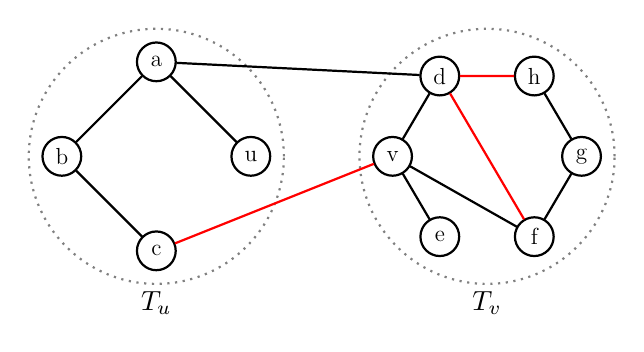
\begin{tikzpicture}
        [scale=0.6, node/.style={scale=0.7, circle,draw,minimum size=2em, thick, font=\large},
        edge/.style={thick, black},
        reserve/.style={red, thick},
        removed/.style={black, thick, dashed}, 
        reserveremoved/.style={red, thick, dashed}]

        \node[node] (u) at (-1,2) {u};
        \node[node] (a) at (-3,4) {a};
        \node[node] (b) at (-5,2) {b};
        \node[node] (c) at (-3,0) {c};
        \node[node] (v) at (2,2) {v};
        \node[node] (d) at (3,3.7) {d};
        \node[node] (e) at (3,0.3) {e};
        \node[node] (f) at (5,0.3) {f};
        \node[node] (g) at (6, 2) {g};
        \node[node] (h) at (5, 3.7) {h};
        
         % Dotted circles for T_u and T_v
        \draw[dotted, thick, gray] (-3,2) circle (2.7cm);
        \draw[dotted, thick, gray] (4,2) circle (2.7cm);  
        
        % Labels for the circles
        \node at (-3,-1.1) {$T_u$};
        \node at (4,-1.1) {$T_v$};

        % tree edges (normal black edges)
        \draw[edge] (a) -- (u) node[midway, below] {};
        \draw[edge] (a) -- (b) node[midway, below] {};
        \draw[edge] (b) -- (c) node[midway, below] {};
        \draw[edge] (v) -- (d) node[midway, below] {};
        \draw[edge] (v) -- (f) node[midway, below] {};
        \draw[edge] (v) -- (e) node[midway, below] {};
        \draw[edge] (f) -- (g) node[midway, below] {};
        \draw[edge] (g) -- (h) node[midway, below] {};
        % reserve edges (normal red edges)
        
        \draw[edge] (a) -- (d) node[midway, below] {};
        \draw[reserve] (c) -- (v) node[midway, below] {};
        \draw[reserve] (d) -- (f) node[midway, below] {};
        \draw[reserve] (d) -- (h) node[midway, below] {};

        \end{tikzpicture}
    \end{minipage}
    \vspace{1cm}
        \noindent
    \begin{minipage}[c]{2cm}
        \raggedright
        Nível $3$
    \end{minipage}%
    \begin{minipage}[c]{0.8\textwidth}
        \centering
        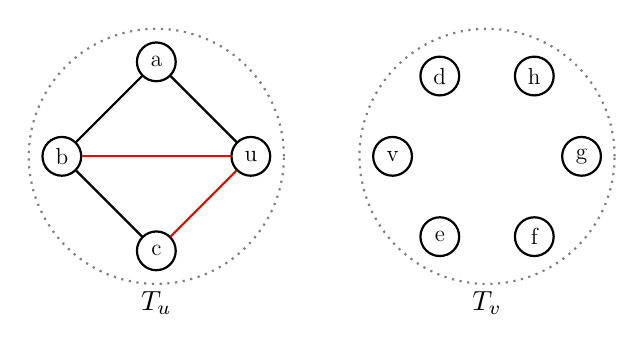
\begin{tikzpicture}
            [scale=0.6, node/.style={scale=0.7, circle,draw,minimum size=2em, thick, font=\large},
            edge/.style={thick, black},
            reserve/.style={red, thick},
            removed/.style={black, thick, dashed}]

            \node[node] (u) at (-1,2) {u};
            \node[node] (a) at (-3,4) {a};
            \node[node] (b) at (-5,2) {b};
            \node[node] (c) at (-3,0) {c};
            \node[node] (v) at (2,2) {v};
            \node[node] (d) at (3,3.7) {d};
            \node[node] (e) at (3,0.3) {e};
            \node[node] (f) at (5,0.3) {f};
            \node[node] (g) at (6, 2) {g};
            \node[node] (h) at (5, 3.7) {h};
            
            
            % Dotted circles for T_u and T_v
            \draw[dotted, thick, gray] (-3,2) circle (2.7cm);
            \draw[dotted, thick, gray] (4,2) circle (2.7cm);  
            
            % Labels for the circles
            \node at (-3,-1.1) {$T_u$};
            \node at (4,-1.1) {$T_v$};
            
            \draw[reserve] (b) -- (u) node[midway, below] {};
            \draw[reserve] (c) -- (u) node[midway, below] {};
            \draw[edge] (a) -- (u) node[midway, below] {};
            \draw[edge] (a) -- (b) node[midway, below] {};
            \draw[edge] (b) -- (c) node[midway, below] {};

        \end{tikzpicture}
    \end{minipage}
    \caption{Representação do grafo com a aresta substituta $ad$ escohida para conectar $T_u$ à $T_v$ em $F_4$, tornando-se uma aresta da floresta.}
    \vspace{-1cm}
    \label{fig:example-replacement4}
\end{figure}

Como essa seção é para dar mais um contexto geral de como a remoção de arestas funciona no grafo dinâmico, optamos por postergar para a Seção~\ref{sec:code-edge-removal} a análise de complexidade de tempo e como as invariantes são preservadas durante a execução do algoritmo, além de mostrar a estratégia usada para percorrer as arestas da floresta e reservas de forma eficiente.  








































\newpage

\section{Implementação do grafo dinâmico}
\label{sec:dynamic-graph-implementation}

\subsection{Construtor}
\label{sec:code-constructor}

Para implementar um grafo dinâmico, chamamos \texttt{grafoDinâmico(n)} para inicializar cada $F_i$ e $R_i$ do grafo $G$ de $n$ vértices, $1 \leq i \leq \left\lceil \lg n \right\rceil$, chamando os métodos \texttt{florestaDinâmica(n)} e \texttt{listaDeAdjacências(n)}, respectivamente. Isso quer dizer que estamos criando florestas dinâmicas e listas de adjacências com $n$ vértices e sem arestas para cada nível $i$. Note que $F_{\left\lceil \lg n \right\rceil}$ e $R_{\left\lceil \lg n \right\rceil}$ representam o grafo dinâmico vazio, sem nenhuma aresta. 

Além disso, usamos um mapa hash para guardar e obter o nível de uma aresta $uv$ em tempo esperado $\Oh(1)$. Assim, este mapa usa como chave os valores das pontas da aresta ($u$ e $v$) e retornam o valor do nível da aresta $uv$. Assim, podemos definir um outro método \texttt{novoMapaHash(n)} que devolve um mapa hash vazio para um grafo de $n$ vértices. Dessa forma, se chamarmos esse método e atribuir a uma variável chamada \textit{nível}, podemos realizar as seguintes operações com \textit{nível}:

\begin{itemize}
    \item \textit{nível[u, v]} $\leftarrow$ i: atribui o nível $i$ a uma aresta $uv$. 
    
    \item \textit{nível[u, v]} $\leftarrow$ \texttt{NIL}: remove a aresta $uv$ e, consequentemente, o seu nível.
    
    \item $x$ $\leftarrow$ \textit{nível[u, v]}: atribui o valor do nível da aresta $uv$ à variável $x$. 
\end{itemize}


Dessa forma, podemos enunciar o construtor do grafo no Programa~\ref{prog:newGD}. 

\begin{programruledcaption}{\texttt{grafoDinâmico(n)} \label{prog:newGD}}
    \noindent\textbf{Entrada}: Recebe um número $n$ de vértices do grafo. \\
    \textbf{Saída}: Devolve um grafo dinâmico $G$ com $n$ vértices e sem arestas.
    \vspace{-0.5\baselineskip}
    \begin{lstlisting}[
        language={[brazilian]pseudocode},
        style=pseudocode,
        style=wider,
        functions={},
        specialidentifiers={},
        escapeinside={(*@}{@*)},
    ]
    \textbf{para} $i$ := $1$ \textbf{até} $\left\lceil \lg n \right\rceil$ \textbf{faça}
        G.$F_i$ := \texttt{florestaDinâmica(n)}
        G.$R_i$ := \texttt{listaDeAdjacências(n)}
    G.nível := \texttt{novoMapaHash(n)}
    devolva G
    \end{lstlisting}
    \vspace{-0.5\baselineskip}
\end{programruledcaption}

Como ambos \texttt{florestaDinâmica(n)} e \texttt{listaDeAdjacências(n)} consomem tempo $\Oh(n)$, então \texttt{grafoDinâmico(n)} consome tempo $\Oh(n \lg n)$, pois estamos criando $\left\lceil \lg n \right\rceil$ florestas dinâmicas e listas de adjacências. Além, disso, as invariantes são mantidas porque estamos criando um grafo com $n$ vértices e sem arestas.

\subsection{Nós do grafo}
\label{sec:graph-nodes}

Como adotamos a técnica de \textit{Euler tour trees} na implementação das nossas florestas dinâmicas, mencionada brevemente na Seção~\ref{sec:dynamic-graph-structure}, estamos utilizando uma estrutura chamada \textbf{nó} que armazena vários atributos relevantes, cuja funcionalidade será descrita mais detalhadamente nas Seções~\ref{sec:code-edge-addition} e \ref{sec:code-edge-removal}. 

Um \textbf{nó} pode representar tanto um vértice da forma $uu$ (ou simplesmente $u$) quanto uma aresta da forma $uv$, $u \neq v$. Em nossa implementação, estaremos usando um mapa hash \textit{nó} para verificar se a entrada \{$u, v$\} existe ou não, retornando um booleano em tempo esperado $\Oh(1)$.

Assim, exclusivamente para cada nó do tipo aresta $uv$, iremos armazenar um atributo booleano chamado \textit{éNível}, que indica se tal aresta pertence a uma floresta maximal de nível $i$. Toda vez que uma aresta nova é inserida no grafo, ela vai ter este atributo definido como verdadeiro. O atributo só se torna falso quando rebaixamos o nível de uma aresta para uma unidade inferior, caso que será descrito em mais detalhes na Seção~\ref{sec:code-edge-removal}. 

Dessa forma, se $uv$ possui nível $2$, então em $F_2$ esse booleano será verdadeiro, e falso em outras $F_i$, $i \neq 2$. Além disso, iremos adicionar um contador \text{arestasDeNível} para cada nó do tipo aresta, a fim de calcular a quantidade de arestas em sua subárvore que tenham o booleano \textit{éNível} como verdadeiro. 

Como o atributo \textit{éNível} pode ser alterado no decorrer das remoções das arestas, precisamos definir uma rotina auxiliar que atualiza o contador \textit{arestasDeNível}, que está descrita no Programa~\ref{prog:updateIsLevelCount-GD}.

\begin{programruledcaption}{\texttt{atualizeArestasDeNível(F, u, v)} \label{prog:updateIsLevelCount-GD}}
    \noindent\textbf{Entrada}: Recebe dois vértices $u$ e $v$ da floresta $F$.
    \vspace{-0.5\baselineskip}
    \begin{lstlisting}[
        language={[brazilian]pseudocode},
        style=pseudocode,
        style=wider,
        functions={},
        specialidentifiers={},
        escapeinside={(*@}{@*)},
    ]
    arestaUV := F.nó[u, v]
    c := 0
    \textbf{se} arestaUV.filhoEsq $\neq$ \texttt{NIL} \textbf{então}
        \textbf{se} arestaUV.filhoEsq.éNível = verdadeiro \textbf{então}
            c := c + 1
    \textbf{se} arestaUV.filhoDir $\neq$ \texttt{NIL} \textbf{então}
        \textbf{se} arestaUV.filhoDir.éNível = verdadeiro \textbf{então}
            c := c + 1
    \textbf{se} arestaUV.éNível = verdadeiro \textbf{então}
        c := c + 1
    arestaUV.arestasDeNível := c
\end{lstlisting}
\vspace{-0.5\baselineskip}
\end{programruledcaption}

Já para o nó do tipo vértice $uu$ (ou apenas $u$), iremos armazenar um booleano chamado \textit{incideArestaReservaDeNível} que indica se $uu$ é uma das pontas de alguma aresta reserva de nível $i$. Dessa forma, se $uv$ é aresta reserva e possui nível $2$, então os vértices $u$ e $v$ em $F_2$ terão \textit{incideArestaReservaDeNível} como verdadeiro. Além disso, iremos manter um contador \textit{arestasReservasDeNível} para cada nó do tipo vértice, a fim de calcular a quantidade de vértices em sua subárvore que tenham o booleano \textit{incideArestaReservaDeNível} como verdadeiro. Esse contador é costantemente atualizado durante as adições e remoções de arestas, e por isso precisamos de um método auxiliar \texttt{atualizeArestasDeNível} descrito no Programa~\ref{prog:updateReserveEdgesCount-GD}.

\begin{programruledcaption}{\texttt{atualizeArestasReservasDeNível(F, u)} \label{prog:updateReserveEdgesCount-GD}}
    \noindent\textbf{Entrada}: Recebe um vértice $u$ da floresta $F$.
    \vspace{-0.5\baselineskip}
    \begin{lstlisting}[
        language={[brazilian]pseudocode},
        style=pseudocode,
        style=wider,
        functions={},
        specialidentifiers={},
        escapeinside={(*@}{@*)},
    ]
    vérticeU := F.nó[u, u]
    c := 0
    \textbf{se} vérticeU.filhoEsq $\neq$ \texttt{NIL} \textbf{então}
        \textbf{se} vérticeU.filhoEsq.incideArestaReservaDeNível = verdadeiro \textbf{então}
            c := c + 1
    \textbf{se} vérticeU.filhoDir $\neq$ \texttt{NIL} \textbf{então}
        \textbf{se} vérticeU.filhoDir.incideArestaReservaDeNível = verdadeiro \textbf{então}
            c := c + 1
    \textbf{se} vérticeU.incideArestaReservaDeNível = verdadeiro \textbf{então}
        c := c + 1
    vérticeU.arestasReservasDeNível := c
    \end{lstlisting}
    \vspace{-0.5\baselineskip}
\end{programruledcaption}
Note que tanto o Programa~\ref{prog:updateIsLevelCount-GD} quando o Programa~\ref{prog:updateReserveEdgesCount-GD} consomem tempo constante $\Oh(1)$, já que ambos envolvem apenas comparações de igualdade e atribuições de valores às variáveis.

Com o Programa~\ref{prog:updateReserveEdgesCount-GD} presente, podemos introduzir dois métodos que modificam o atributo \textit{incideArestaReservaDeNível} e atualizam o contador \textit{arestasReservasDeNível}.

\begin{programruledcaption}{\texttt{decrementeArestasReservasDeNível(F, L, u)} \label{prog:decrementReserveEdgesCount-GD}}
    \noindent\textbf{Entrada}: Recebe um vértice $u$ da floresta $F$ e uma lista de adjacências $L$.
    \vspace{-0.5\baselineskip}
    \begin{lstlisting}[
        language={[brazilian]pseudocode},
        style=pseudocode,
        style=wider,
        functions={},
        specialidentifiers={},
        escapeinside={(*@}{@*)},
        ]
        vérticeU := F.nó[u, u]
        \textbf{se} L[u] = $\emptyset$ \textbf{então} 
        \texttt{puxeParaRaiz(F, vérticeU)}
        vérticeU.incideArestaReservaDeNível = falso
        \texttt{atualizeIncideArestaReservaDeNível(F, u)}
    \end{lstlisting}
    \vspace{-0.5\baselineskip}
\end{programruledcaption}


No Programa~\ref{prog:decrementReserveEdgesCount-GD}, atualizamos o atributo \textit{incideArestaReservaDeNível} de um vértice $u$ para falso quando ele não tiver mais vizinhos, visto que não haverá mais nenhuma aresta reserva incidente nele. A assinatura \texttt{L[u]} retorna o conjunto de vizinhos do vértice $u$. A rotina auxiliar \texttt{puxeParaRaiz} serve apenas para propagar corretamente a atualização deste atributo nos outros nós que estão conectados com $u$. Como estamos usando uma \textit{splay tree}, então puxar o vértice $u$ para a raiz consome tempo amortizado O(lg$n$). Já a rotina auxiliar \texttt{atualizeIncideArestaReservaDeNível} no Programa~\ref{prog:updateReserveEdgesCount-GD} apenas atualiza o atributo \textit{arestasReservasDeNível}, consumindo tempo $\Oh(1)$. Dessa forma, \texttt{decrementeArestasReservasDeNível} consome tempo amortizado O(lg$n$).

\begin{programruledcaption}{\texttt{incrementeArestasReservasDeNível(F, L, u)} \label{prog:incrementReserveEdgesCount-GD}}
    \noindent\textbf{Entrada}: Recebe um vértice $u$ da floresta $F$ e uma lista de adjacências $L$.
    \vspace{-0.5\baselineskip}
    \begin{lstlisting}[
        language={[brazilian]pseudocode},
        style=pseudocode,
        style=wider,
        functions={},
        specialidentifiers={},
        escapeinside={(*@}{@*)},
    ]
    vérticeU := F.nó[u, u]
    \textbf{se} |L[u]| = $1$ \textbf{então} 
        \texttt{puxeParaRaiz(F, vérticeU)}
        vérticeU.incideArestaReservaDeNível = verdadeiro
        \texttt{atualizeIncideArestaReservaDeNível(F, u)}
    \end{lstlisting}
    \vspace{-0.5\baselineskip}
\end{programruledcaption}

Por fim, o Programa~\ref{prog:incrementReserveEdgesCount-GD} atualiza o atributo \textit{incideArestaReservaDeNível} de um vértice $u$ para verdadeiro quando adicionamos um vértice $v$ na lista de adjacências de $u$ (assumindo que $u$ não tinha nenhum vizinho antes), pois isso indica que $u$ é incidente à aresta reserva $uv$. Da mesma forma que o Programa~\ref{prog:decrementReserveEdgesCount-GD}, o método \texttt{incrementeArestasReservasDeNível} possui consumo de tempo amortizado O(lg$n$).

Como essas rotinas auxiliares não fazem nenhuma modificação na floresta maximal do grafo, então todas as invariantes não mantidas.

\subsection{Teste de conexidade entre dois vértices}
\label{sec:code-connectivity-test}

Como mostrado na Seção~\ref{sec:dynamic-graph-structure}, ao chamarmos o método \texttt{conectadosGD} estamos na verdade testando a conexidade na floresta maximal $F_{\left\lceil \lg n \right\rceil}$ de $G$, ou seja, estamos chamando a rotina \texttt{conectadosFD}. O invariante \ref{invariant1} garante que $F_{\left\lceil \lg n \right\rceil}$ é uma floresta maximal de $G$, e, portanto, consultas em 
\texttt{conectadosFD($F_{\left\lceil \lg n \right\rceil}$, u, v)} deveriam dar a mesma resposta que \texttt{conectadosGD(G, u, v)}, onde $G$ = $G_{\left\lceil \lg n \right\rceil}$. Dessa forma, podemos enunciar essa rotina no Programa~\ref{prog:connectedGD}.

\begin{programruledcaption}{\texttt{conectadosGD(G, u, v)} \label{prog:connectedGD}}
    \noindent\textbf{Entrada}: Recebe dois vértices $u$ e $v$ do grafo $G$. \\
    \textbf{Saída}: Devolve um booleano indicando se $u$ e $v$ estão conectados em $G$.
    \vspace{-0.5\baselineskip}
    \begin{lstlisting}[
        language={[brazilian]pseudocode},
        style=pseudocode,
        style=wider,
        functions={},
        specialidentifiers={},
        escapeinside={(*@}{@*)},
    ]
    devolva \texttt{conectadosFD($G.F_{\left\lceil \lg n \right\rceil}$, u, v)}
    \end{lstlisting}
    \vspace{-0.5\baselineskip}
\end{programruledcaption}

O consumo de tempo de \texttt{conectadosGD} é amortizado O(lg$n$), visto que ele simplesmente chama \texttt{conectadosFD} que tem consumo amortizado O(lg$n$). Além disso, a rotina de consulta não altera o nosso grafo, incluindo florestas e listas de adjacências, já que não há nenhuma modificação neles. Isso implica que as invariantes são mantidas. 

\subsection{Adição de arestas}
\label{sec:code-edge-addition}

Se quisermos inserir uma aresta $uv$ no grafo $G$, basta chamarmos o método \texttt{adicioneGD(G, u, v)}. Entretanto, antes de adicionar na floresta maximal $F_{\left\lceil \lg n \right\rceil}$ de $G$, chamamos antes a rotina \texttt{conectadosFD($F_{\left\lceil \lg n \right\rceil}$, u, v)} para verificar se $u$ e $v$ já estão conectados. Se sim, então $uv$ será armazenada como aresta reserva em $R_{\left\lceil \lg n \right\rceil}$. Se os vértices $u$ e $v$ não estiverem conectados, então adicionamos a aresta $uv$ em $F_{\left\lceil \lg n \right\rceil}$. O Programa~\ref{prog:addGD} ilustra a rotina \texttt{adicioneGD}.

\begin{programruledcaption}{\texttt{adicioneGD(G, u, v)} \label{prog:addGD}}
    \noindent\textbf{Entrada}: Recebe dois vértices $u$ e $v$ do grafo $G$. \\
    \textbf{Saída}: Devolve o grafo $G$ com a aresta $uv$ inserida.
    \vspace{-0.5\baselineskip}
    \begin{lstlisting}[
        language={[brazilian]pseudocode},
        style=pseudocode,
        style=wider,
        functions={},
        specialidentifiers={},
        escapeinside={(*@}{@*)},
    ]
    G.nível[u, v] := $\left\lceil \lg n \right\rceil$
    \textbf{se} \texttt{conectadosFD(G.$F_{\left\lceil \lg n \right\rceil}$, u, v)} \textbf{então}
        \texttt{adicioneLA(G.$R_{\left\lceil \lg n \right\rceil}$, u, v)}
        \texttt{incrementeArestasReservasDeNível(G.$F_{\left\lceil \lg n \right\rceil}$, G.$R_{\left\lceil \lg n \right\rceil}$, u)}
        \texttt{incrementeArestasReservasDeNível(G.$F_{\left\lceil \lg n \right\rceil}$, G.$R_{\left\lceil \lg n \right\rceil}$, v)}
    \textbf{senão}
        \texttt{adicioneFD(G.$F_{\left\lceil \lg n \right\rceil}$, u, v)}
    devolva G
    \end{lstlisting}
    \vspace{-0.5\baselineskip}
\end{programruledcaption}

Ao inserirmos uma aresta reserva $uv$ em $G$, precisamos atualizar o atributo \textit{incideArestaReservaDeNível} de $u$ e de $v$ para verdadeiro, se necessário. A Seção~\ref{sec:graph-nodes} explica com mais detalhes o método auxiliar (\texttt{incrementeArestasReservasDeNível}) usado. 

A invariante \ref{invariant1} se mantém para o nível $i = \left\lceil \lg n \right\rceil$. Como sempre adicionamos arestas em $F_{\left\lceil \lg n \right\rceil}$ (se não forem reservas), então as outras florestas de níveis inferiores não são afetadas, mantendo-se, assim, os invariantes \ref{invariant2} e \ref{invariant3} também.

Como o consumo de tempo de \texttt{conectadosFD}, \texttt{adicioneFD} e de \texttt{incrementeArestasReservasDeNível} é amortizado O(lg$n$), e \texttt{adicioneLA} possui custo esperado $\Oh(1)$, então temos que \texttt{adicioneGD} possui consumo de tempo amortizado O(lg$n$).

\subsection{Remoção de arestas}
\label{sec:code-edge-removal}

Como mencionado na Seção~\ref{sec:dynamic-graph-edge-removal}, encontramos duas situações ao removermos uma aresta $uv$ de um grafo $G$. A mais simples é quando a que queremos resolver é uma reserva, pois basta removermos da lista de adjacências de $G$. Porém, quando removemos uma aresta da floresta, podemos acabar quebrando ela em duas componentes, $T_u$ e $T_v$, e precisamos procurar uma aresta substituta que conecte as duas. O Programa~\ref{prog:removeGD} ilustra o método \texttt{removaGD}.

\begin{programruledcaption}{\texttt{removaGD(G, u, v)} \label{prog:removeGD}}
    \noindent\textbf{Entrada}: Recebe dois vértices $u$ e $v$ do grafo $G$. \\
    \textbf{Saída}: Devolve o grafo $G$ com a aresta $uv$ removida.
    \vspace{-0.5\baselineskip}
    \begin{lstlisting}[
        language={[brazilian]pseudocode},
        style=pseudocode,
        style=wider,
        functions={},
        specialidentifiers={},
        escapeinside={(*@}{@*)},
    ]
    i := G.nível[u, v]
    nível[u, v] := NIL // marcamos uv como removida
    \textbf{se} uv $\in$ G.$F_{\left\lceil \lg n \right\rceil}$ \textbf{então}
        \textbf{para} j := i \textbf{até} $\left\lceil \lg n \right\rceil$ \textbf{faça}
            \texttt{removaFD($G.F_j$, u, v)}
        \texttt{substituaAresta(G, i, u, v)}
    \textbf{senão}
        \texttt{removaLA($G.R_i$, u, v)}
        \texttt{decrementeArestasReservasDeNível($G.F_i$, $G.R_i$, u)}
        \texttt{decrementeArestasReservasDeNível($G.F_i$, $G.R_i$, v)}
    devolva G
    \end{lstlisting}
    \vspace{-0.5\baselineskip}
\end{programruledcaption}

Ao remover uma aresta $uv$ de nível $i$ de $G$, precisamos conferir se ela pertence à floresta $F_{\left\lceil \lg n \right\rceil}$ (linha $3$ do Programa~\ref{prog:removeGD}). Para isso, podemos utilizar um método auxiliar como em Programa~\ref{prog:existGD}, que retorna um booleano indicando se o nó $uv$ existe ou não.

\begin{programruledcaption}{\texttt{existeNoGrafo(F, u, v)} \label{prog:existGD}}
    \noindent\textbf{Entrada}: Recebe dois vértices $u$ e $v$ do grafo $G$. \\
    \textbf{Saída}: Devolve um booleano indicando se a aresta $uv$ existe em $G$.
    \vspace{-0.5\baselineskip}
    \begin{lstlisting}[
        language={[brazilian]pseudocode},
        style=pseudocode,
        style=wider,
        functions={},
        specialidentifiers={},
        escapeinside={(*@}{@*)},
    ]
    devolva F.nó[u, v] $\neq \emptyset$ 
    \end{lstlisting}
    \vspace{-0.5\baselineskip}
\end{programruledcaption}

Se $uv$ não é uma aresta da floresta, então ela é reserva e basta removê-la de $R_i$ (linha $8$ do Programa~\ref{prog:removeGD}) em tempo esperado $\Oh(1)$. Entretanto, quando removemos uma aresta $uv$, pode ocorrer o caso em que $u$ (ou $v$) não seja mais incidente a alguma outra aresta reserva, por isso precisamos atualizar o contador \textit{arestasReservasDeNível} tanto de $u$ quanto de $v$ chamando a rotina auxiliar \texttt{decrementeArestasReservasDeNível} do Programa~\ref{prog:decrementReserveEdgesCount-GD}.

Já para o caso em que $uv$ é uma aresta da floresta, precisamos removê-la das florestas $F_j$, $F_{j+1}, \ldots, F_{\left\lceil \lg n \right\rceil}$, para $i \leq j \leq \left\lceil \lg n \right\rceil$, onde $i$ é o nível de $uv$. Essa remoção é feita na linha $5$ chamando a rotina \texttt{removaFD}. Essa remoção é necessária devido à invariante~\ref{invariant2}, pois sabemos que $uv$ está somente nas florestas desses níveis. 

O laço da linha $4$ no Programa~\ref{prog:removeGD} executa no pior dos casos O(lg$n$) vezes, e como \texttt{removaFD} consome tempo amortizado O(lg$n$), então as linhas $4$ e $5$ do código juntas possuem um consumo de tempo esperado $\Oh(n \lg 2^n)$. Como vimos que \texttt{removaLA} tem consumo esperado de tempo $\Oh(1)$ e \texttt{decrementeArestasReservasDeNível} consome tempo amortizado O(lg$n$), então o trecho do código que abrange as linhas 8 a 10 tem custo amortizado O(lg$n$). Por fim, veremos que a rotina auxiliar \texttt{substituaAresta} terá custo amortizado $\Oh(n \lg 2^n)$, concluindo-se então que \texttt{removaGD} consome tempo amortizado $\Oh(n \lg 2^n)$. Essa rotina auxiliar é a mais complexa do grafo dinâmico, e ela está descrita no descrita no Programa~\ref{prog:replaceGD}.

\begin{programruledcaption}{\texttt{substituaAresta(G, i, u, v)} \label{prog:replaceGD}}
    \noindent\textbf{Entrada}: Recebe dois vértices $u$ e $v$ do grafo $G$, e o nível $i$ da aresta $uv$.
    \vspace{-0.5\baselineskip}
    \begin{lstlisting}[
        language={[brazilian]pseudocode},
        style=pseudocode,
        style=wider,
        functions={},
        specialidentifiers={},
        escapeinside={(*@}{@*)},
    ]
    \textbf{para} j := i \textbf{até} $\left\lceil \lg n \right\rceil$ \textbf{faça}
        $T_u$ := \texttt{árvore($F_j$.nó[u, u])}
        $T_v$ := \texttt{árvore($F_j$.nó[v, v])}    
        \textbf{se} |$T_u$| > |$T_v$| \textbf{então}
            u $\leftrightarrow$ v
            $T_u \leftrightarrow T_v$
        \textbf{para} $xy$ $\in$ $T_u$ \textbf{e} G.nível[x, y] = j \textbf{faça} // rebaixa o nível das arestas de $T_u$ para $j-1$
            G.nível[x, y] := j - 1
            \texttt{adicioneFD($G.F_{j-1}$, x, y)}
            arestaXY := $F_j$.nó[x, y]
            \texttt{puxeParaRaiz(arestaXY)}
            arestaXY.éNível := falso
            \texttt{atualizeNívelDeAresta($F_j$, x, y)}
        \textbf{para} $xy$ $\in G.R_j$ \textbf{e} x $\in T_u$ \textbf{faça} // procura aresta substituta que ligue $T_u$ e $T_v$
            \texttt{removaLA($G.R_j$, x, y)} 
            \textbf{se} $y \in T_v$ \textbf{então} // achamos uma aresta substituta $xy$
                \textbf{para} k := j \textbf{até} $\left\lceil \lg n \right\rceil$ \textbf{faça}
                    \texttt{adicioneFD($G.F_k$, x, y)}
                \textbf{devolva}
            \textbf{senão}
                G.nível[x, y] := j - 1
                \texttt{adicioneLA($G.R_{j-1}$, x, y)}
                \texttt{incrementeArestasReservasDeNível($G.F_{j-1}$, $G.R_{j-1}$, x)}
                \texttt{incrementeArestasReservasDeNível($G.F_{j-1}$, $G.R_{j-1}$, y)}

    \end{lstlisting}
    \vspace{-0.5\baselineskip}
\end{programruledcaption}

Para explicar o Programa~\ref{prog:replaceGD}, iremos usar imagens para ilustrar o que está acontecendo em cada trecho do código. Como já comentado na Seção~\ref{sec:dynamic-graph-edge-removal}, ao removermos uma única aresta $uv$ que conecta $T_u$ e $T_v$, que contêm, respectivamente, o vértice $u$ e $v$, quebramos a floresta em duas componentes $T_u$ e $T_v$. Na Figura~\ref{fig:example-removal-part1}, a floresta de nível $i$ mostra um exemplo em que a aresta da floresta $uv$ é removida da floresta de nível $i$, separando-a em duas árvores $T_u$ e $T_v$. Já a floresta de nível $i-1$ no momento contém apenas vértice isolados.

Denotando $|T|$ como o número de vértices de uma árvore $T$, podemos, sem perda de generalidade, assumir que $|T_u| \leq |T_v|$. Pela invariante~\ref{invariant3}, temos que $|T| \leq 2^i$, e como $|T_u| + |T_v| = |T|$, então $|T_u| \leq 2^{i-1}$. Por isso, podemos rebaixar todas as arestas de nível $i$ de $|T_u|$ para o nível $i-1$, mantendo-se, assim, a invariante~\ref{invariant3}. 

\begin{figure}[H]
    \centering

    \noindent
    \begin{minipage}[c]{2cm}
        \raggedright
        Nível $i$
    \end{minipage}%
    \begin{minipage}[c]{0.8\textwidth}
        \centering
        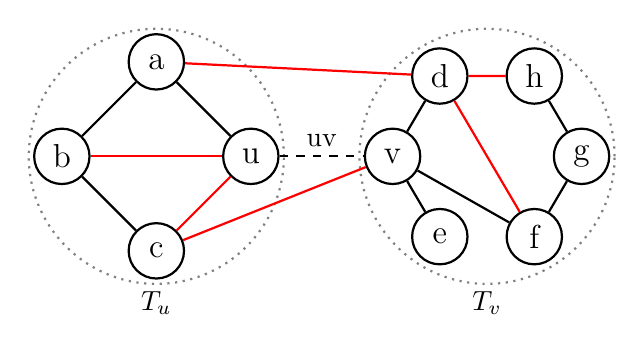
\begin{tikzpicture}
        [scale=0.6, node/.style={circle,draw,minimum size=2em, thick, font=\large},
        edge/.style={thick, black},
        reserve/.style={red, thick},
        removed/.style={black, thick, dashed}]

        \node[node] (u) at (-1,2) {u};
        \node[node] (a) at (-3,4) {a};
        \node[node] (b) at (-5,2) {b};
        \node[node] (c) at (-3,0) {c};
        \node[node] (v) at (2,2) {v};
        \node[node] (d) at (3,3.7) {d};
        \node[node] (e) at (3,0.3) {e};
        \node[node] (f) at (5,0.3) {f};
        \node[node] (g) at (6, 2) {g};
        \node[node] (h) at (5, 3.7) {h};
        
        
         % Dotted circles for T_u and T_v
        \draw[dotted, thick, gray] (-3,2) circle (2.7cm);
        \draw[dotted, thick, gray] (4,2) circle (2.7cm);  
        
        % Labels for the circles
        \node at (-3,-1.1) {$T_u$};
        \node at (4,-1.1) {$T_v$};

        % tree edges (normal black edges)
        \draw[edge] (a) -- (u) node[midway, below] {};
        \draw[edge] (a) -- (b) node[midway, below] {};
        \draw[edge] (b) -- (c) node[midway, below] {};
        \draw[edge] (v) -- (d) node[midway, below] {};
        \draw[edge] (v) -- (f) node[midway, below] {};
        \draw[edge] (v) -- (e) node[midway, below] {};
        \draw[removed] (u) -- (v) node[midway, above] {uv};
        \draw[edge] (f) -- (g) node[midway, below] {};
        \draw[edge] (g) -- (h) node[midway, below] {};
        % reserve edges (normal red edges)

        \draw[reserve] (a) -- (d) node[midway, below] {};
        \draw[reserve] (c) -- (v) node[midway, below] {};
        \draw[reserve] (b) -- (u) node[midway, below] {};
        \draw[reserve] (c) -- (u) node[midway, below] {};
        \draw[reserve] (d) -- (f) node[midway, below] {};
        \draw[reserve] (d) -- (h) node[midway, below] {};

        \end{tikzpicture}
    \end{minipage}
    \vspace{1cm}
        \noindent
    \begin{minipage}[c]{2cm}
        \raggedright
        Nível $i - 1$
    \end{minipage}%
    \begin{minipage}[c]{0.8\textwidth}
        \centering
        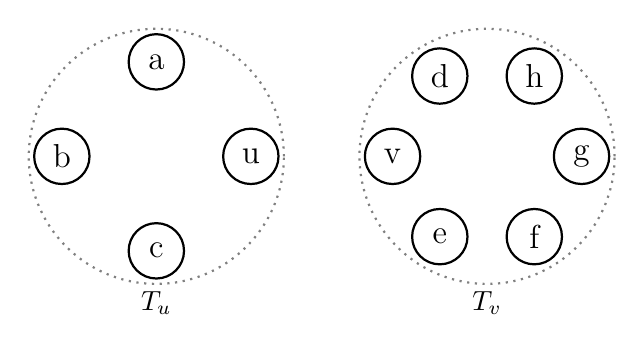
\begin{tikzpicture}
            [scale=0.6, node/.style={circle,draw,minimum size=2em, thick, font=\large},
            edge/.style={thick, black},
            reserve/.style={red, thick},
            removed/.style={black, thick, dashed}]

            \node[node] (u) at (-1,2) {u};
            \node[node] (a) at (-3,4) {a};
            \node[node] (b) at (-5,2) {b};
            \node[node] (c) at (-3,0) {c};
            \node[node] (v) at (2,2) {v};
            \node[node] (d) at (3,3.7) {d};
            \node[node] (e) at (3,0.3) {e};
            \node[node] (f) at (5,0.3) {f};
            \node[node] (g) at (6, 2) {g};
            \node[node] (h) at (5, 3.7) {h};
            
            
            % Dotted circles for T_u and T_v
            \draw[dotted, thick, gray] (-3,2) circle (2.7cm);
            \draw[dotted, thick, gray] (4,2) circle (2.7cm);  
            
            % Labels for the circles
            \node at (-3,-1.1) {$T_u$};
            \node at (4,-1.1) {$T_v$};

        \end{tikzpicture}
    \end{minipage}
    \caption{As arestas pretas são da floresta, enquanto as vermelhas são reservas. A aresta $uv$ tracejada está prestes a ser removida. A floresta de cima é de nível i, enquanto a de baixo é de nível i - 1.}
    \vspace{-1cm}
    \label{fig:example-removal-part1}
\end{figure}

No Programa~\ref{prog:replaceGD}, o rebaixamento das arestas é feito nas linhas $7$ ao $13$ do código. Na linha $7$, percorremos todas as arestas de $T_u$ que são de nível $i$. Assim, para cada aresta de nível $i$, atualizamos o nível delas para $i - 1$. Quando rebaixamos as arestas de nível $i$ de $F_i$, elas se tornarão arestas da floresta $F_{i-1}$. 

Alem disso, note que, após o rebaixamento, essas arestas não são mais de nível $i$ em $F_i$, e portanto precisamos atualizar o atributo \textit{éNível} delas para falso em $F_i$ (em $F_{i-1}$ elas automaticamente já terão o \textit{éNível} definido como verdadeiro), e consequentemente atualizamos o contador \textit{arestasDeNível} chamando a função auxiliar \texttt{atualizeArestasDeNível} do Programa~\ref{prog:updateIsLevelCount-GD}.  


O Programa~\ref{fig:example-removal-part2} ilustra o rebaixamento das arestas no grafo.

\begin{figure}[H]
    \centering

    \noindent
    \begin{minipage}[c]{2cm}
        \raggedright
        Nível $i$
    \end{minipage}%
    \begin{minipage}[c]{0.8\textwidth}
        \centering
        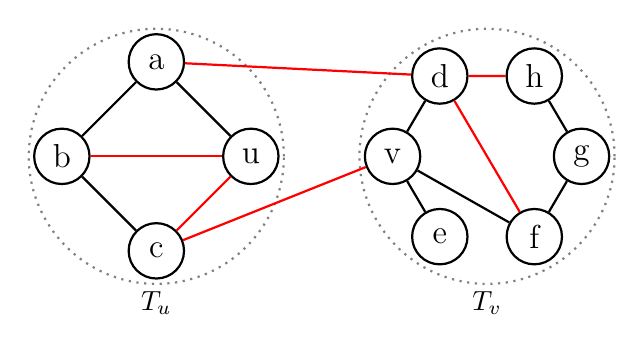
\begin{tikzpicture}
        [scale=0.6, node/.style={circle,draw,minimum size=2em, thick, font=\large},
        edge/.style={thick, black},
        reserve/.style={red, thick},
        removed/.style={black, thick, dashed}]

        \node[node] (u) at (-1,2) {u};
        \node[node] (a) at (-3,4) {a};
        \node[node] (b) at (-5,2) {b};
        \node[node] (c) at (-3,0) {c};
        \node[node] (v) at (2,2) {v};
        \node[node] (d) at (3,3.7) {d};
        \node[node] (e) at (3,0.3) {e};
        \node[node] (f) at (5,0.3) {f};
        \node[node] (g) at (6, 2) {g};
        \node[node] (h) at (5, 3.7) {h};
        
        
         % Dotted circles for T_u and T_v
        \draw[dotted, thick, gray] (-3,2) circle (2.7cm);
        \draw[dotted, thick, gray] (4,2) circle (2.7cm);  
        
        % Labels for the circles
        \node at (-3,-1.1) {$T_u$};
        \node at (4,-1.1) {$T_v$};

        % tree edges (normal black edges)
        \draw[edge] (a) -- (u) node[midway, below] {};
        \draw[edge] (a) -- (b) node[midway, below] {};
        \draw[edge] (b) -- (c) node[midway, below] {};
        \draw[edge] (v) -- (d) node[midway, below] {};
        \draw[edge] (v) -- (f) node[midway, below] {};
        \draw[edge] (v) -- (e) node[midway, below] {};
        \draw[edge] (f) -- (g) node[midway, below] {};
        \draw[edge] (g) -- (h) node[midway, below] {};
        % reserve edges (normal red edges)

        \draw[reserve] (a) -- (d) node[midway, below] {};
        \draw[reserve] (c) -- (v) node[midway, below] {};
        \draw[reserve] (b) -- (u) node[midway, below] {};
        \draw[reserve] (c) -- (u) node[midway, below] {};
        \draw[reserve] (d) -- (f) node[midway, below] {};
        \draw[reserve] (d) -- (h) node[midway, below] {};

        \end{tikzpicture}
    \end{minipage}
    \vspace{1cm}
        \noindent
    \begin{minipage}[c]{2cm}
        \raggedright
        Nível $i - 1$
    \end{minipage}%
    \begin{minipage}[c]{0.8\textwidth}
        \centering
        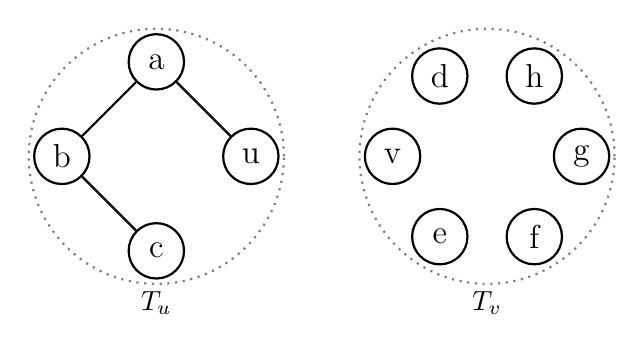
\begin{tikzpicture}
            [scale=0.6, node/.style={circle,draw,minimum size=2em, thick, font=\large},
            edge/.style={thick, black},
            reserve/.style={red, thick},
            removed/.style={black, thick, dashed}]

            \node[node] (u) at (-1,2) {u};
            \node[node] (a) at (-3,4) {a};
            \node[node] (b) at (-5,2) {b};
            \node[node] (c) at (-3,0) {c};
            \node[node] (v) at (2,2) {v};
            \node[node] (d) at (3,3.7) {d};
            \node[node] (e) at (3,0.3) {e};
            \node[node] (f) at (5,0.3) {f};
            \node[node] (g) at (6, 2) {g};
            \node[node] (h) at (5, 3.7) {h};
            
            
            % Dotted circles for T_u and T_v
            \draw[dotted, thick, gray] (-3,2) circle (2.7cm);
            \draw[dotted, thick, gray] (4,2) circle (2.7cm);  
            
            % Labels for the circles
            \node at (-3,-1.1) {$T_u$};
            \node at (4,-1.1) {$T_v$};
            
            \draw[edge] (a) -- (u) node[midway, below] {};
            \draw[edge] (a) -- (b) node[midway, below] {};
            \draw[edge] (b) -- (c) node[midway, below] {};

        \end{tikzpicture}
    \end{minipage}
    \caption{As arestas pretas são da floresta, enquanto as vermelhas são reservas. A aresta $uv$ já foi removida removida. A floresta de cima é de nível i, enquanto a de baixo é de nível i - 1, com as arestas de nível i rebaixadas.}
    \vspace{-1cm}
    \label{fig:example-removal-part2}
\end{figure}

%!TeX root=../tese.tex
%("dica" para o editor de texto: este arquivo é parte de um documento maior)
% para saber mais: https://tex.stackexchange.com/q/78101

\chapter{Conexidade em grafos dinâmicos}

\enlargethispage{.8\baselineskip}

\section{Definição}

Como citado no Capítulo 1, o problema da conexidade em grafos dinâmicos visa construir um algoritmo eficiente para a seguinte biblioteca, que contém:

\begin{itemize}
    \item \texttt{\textbf{grafoDinâmico(G, n)}}: devolve um grafo dinâmico $G$ com $n$ vértices isolados;
    \item \texttt{\textbf{conectado(G, u, v)}}: devolve verdadeiro se os vértices $u$ e $v$ estão na mesma componente de $G$ e falso caso contrário;
    \item \texttt{\textbf{adiciona(G, u, v)}}: adiciona a aresta $uv$ no grafo $G$;
    \item \texttt{\textbf{remova(G, u, v)}}: remove a aresta $uv$ do grafo $G$.
\end{itemize} 

O algoritmo de Holm, de Lichtenberg e Thorup para este problema de conexidade é composto por $\left\lceil \lg n \right\rceil$ florestas dinâmicas do grafo $G$, que utilizam o algoritmo mencionado na Seção 2. Cada aresta do grafo possui um nível entre $0$ e $\left\lceil \lg n \right\rceil$. O nível inicial de uma aresta recém-inserida é sempre $\left\lceil \lg n \right\rceil$, e ele nunca aumenta, apenas diminui. Assim, cada aresta de nível $i$ pertence à floresta dinâmica de mesmo nível. 

Ademais, a consulta \texttt{conectado(u, v)} aplicada ao grafo $G$ significa fazer a mesma consulta para alguma floresta maximal $F$ de $G$. Dessa maneira, sempre que estivermos realizando alguma operação de alteração ou consulta de conexidade em nosso grafo $G$, estamos realizando-a em uma floresta dinâmica $F$ que seja maximal em $G$. Da mesma forma, quando chamamos o construtor do grafo dinâmico, estamos criando $\lg n$ florestas de vértices isolados.

%%%%%%%%%%%%%%% SEÇÕES FINAIS (BIBLIOGRAFIA E ÍNDICE REMISSIVO) %%%%%%%%%%%%%%%%

% O comando backmatter desabilita a numeração de capítulos.
\backmatter

\pagestyle{backmatter}

% Espaço adicional no sumário antes das referências / índice remissivo
%\addtocontents{toc}{\vspace{2\baselineskip plus .5\baselineskip minus .5\baselineskip}}

% A bibliografia é obrigatória

\printbibliography[
  %title=\refname\label{sec:bib}, % "Referências", recomendado pela ABNT
  title=\bibname\label{sec:bib}, % "Bibliografia"
  heading=bibintoc, % Inclui a bibliografia no sumário
]

%\printindex % imprime o índice remissivo no documento (opcional)

\end{document}
